% !TEX TS-program = pdflatex
% !TEX encoding = UTF-8 Unicode

\documentclass[12pt,oneside,letterpaper]{article}

% release codenumber (update it here!)
\newcommand\releasecode{0.3.0}

%%% PACKAGES
\usepackage{lmodern} % Activa fuentes y macros de Latin Modern
\usepackage[T1]{fontenc} % set font encoding
\usepackage[utf8]{inputenc} % set input encoding (not needed with XeLaTeX)
\usepackage[english]{babel} 
\usepackage[expert, charter]{mathdesign} % Fuentes... disponibles conjuntos {charter|utopia}
%%\usepackage{calligra}
\usepackage[printwatermark]{xwatermark}
\usepackage{graphicx}
\usepackage[usenames,dvipsnames,table]{xcolor}
\usepackage{parskip}
%%\usepackage{float}
%\usepackage[nolists,tablesfirst, nomarkers]{endfloat}
\usepackage{moreverb} % for verbatim output

% text layout
\usepackage[letterpaper]{geometry}
\geometry{textwidth=16.25cm} % 15.25cm for single-space, 16.25cm for double-space
\geometry{textheight=22.5cm} % 22cm for single-space, 22.5cm for double-space

% watermarks (time consuming!)
\newwatermark[allpages,color=PineGreen!4,angle=45,scale=9,xpos=-40,ypos=0]{DRAFT}
\newwatermark[allpages,color=PineGreen!12,angle=0,scale=1,xpos=0,ypos=137]{
\emph{mSystems} \LaTeX\ manuscript release \releasecode}

% helps to keep figures from being orphaned on a page by themselves
\renewcommand{\topfraction}{0.85}
\renewcommand{\textfraction}{0.1}
%% Roman footnote numbering style to not collide with bibliographic cites: 
\renewcommand{\thefootnote}{\Roman{footnote}}

% line numbering
\usepackage[running,mathlines]{lineno}
\renewcommand\thelinenumber{\color{red}\arabic{linenumber}}
\linenumbers

% bold the 'Figure #' in the caption and separate it with a period
% Captions will be left justified
\usepackage[labelfont=bf,labelsep=period,font=small]{caption}

% review layout with double-spacing
\usepackage{setspace} 
\captionsetup{labelfont=bf,labelsep=period,font=doublespacing}

% cite package, to clean up citations in the main text. Do not remove.
\usepackage{cite}
\renewcommand\citeleft{(}
\renewcommand\citeright{)}
\renewcommand\citeform[1]{\textsl{#1}}

% Remove brackets from numbering in list of References
\renewcommand\refname{\large References}
\makeatletter
\renewcommand{\@biblabel}[1]{\quad#1.}
\makeatother

% Importance environment and keywords command
\newcommand\importancename{Importance}
\newcommand{\importance}[1]{
	{
    \small
    \begin{center}
        {\bfseries \importancename\vspace{-.5em}\vspace{0pt}}
    \end{center}
    \begin{quote}
    #1
    \end{quote}
    }
}
\providecommand{\keywords}[1]{\footnotesize\textbf{\textit{Keywords---}} #1}

% Package authblk
\usepackage{authblk}
\renewcommand\Authands{ \& }
\renewcommand\Authfont{\normalsize \bf}
\renewcommand\Affilfont{\small \normalfont}

% notation
\usepackage{amsmath}

%% Roman footnote numbering style to not collide with bibliographic cites: 
\renewcommand{\thefootnote}{\Roman{footnote}}

% aux commands
\newcommand{\CC}[0]{\emph{cmplxcruncher}}
\newcommand{\task}[1]{\texttt{\bfseries\scshape\textcolor{MidnightBlue}{#1}}}
\newcommand{\un}[1]{\operatorname{#1}}
\newcommand{\unclassrate}[0]{\un{kpb/s/core}}
\newcommand{\todo}[1]{\texttt{\bfseries\textcolor{Orange}{#1}}}


% word count (Need --enable-write18 or --shell-escape)
\immediate\write18{texcount -opt=option.tc \jobname.tex > wordcount.aux} 
\newcommand\wordcount{\verbatiminput{wordcount.aux}}


%%% DOCUMENT %%%

\begin{document}

\title{
	\vspace*{0mm} % May help to include the corresponding author footnote in the title page
	\singlespacing
	\begin{flushleft}
		\texttt{\large Title:} \\
	\end{flushleft}
	\vspace*{2mm}
	Health and disease imprinted in the time variability of the human microbiome\\
	\vspace*{6mm}
	\begin{flushleft}
		\texttt{\large Running title:} \\
	\end{flushleft}
	\vspace*{0mm}
	Microbiota, are you sick?
	\vspace*{4mm}
	}

\doublespacing

\author[1,2,$*$]{Jose Manuel Martí}
\author[1,2,3,$*$]{Daniel Martínez-Martínez}
\author[2]{Manuel Peña}
\author[1,2]{César Gracia}
\author[1,3,4,5]{Amparo Latorre}
\author[1,3,4,5,\#]{Andrés Moya}
\author[1,2,\#]{Carlos P. Garay}

\affil[1]{Institute for Integrative Systems Biology (I2SysBio), 46980, Spain.}
\affil[2]{Instituto de Fisica Corpuscular, CSIC-UVEG, P.O.  22085, 46071, Valencia, Spain.}
\affil[3]{FISABIO, Avda de Catalunya, 21, 46020, Valencia, Spain.}
\affil[4]{Cavanilles Institute of Biodiversity and Evolutionary Biology, UVEG, 46980, Spain.}
\affil[5]{CIBER en Epidemiología y Salud Pública (CIBEResp), Madrid, Spain}

\date{}

\maketitle
\wordcount
\footnote[0]{$^*$ Equally contributed}
\footnote[0]{$^\#$ Corresponding authors: andres.moya@uv.es, penagaray@gmail.com}

\clearpage

%TC:newcounter abswords Words in abstract
%TC:macro \abstract [abswords]
{\abstract{Animal microbiota (human included) plays an important role keeping healthy the physiological status of the host. Increasing research activity is dedicated to understand how changes in composition and function of the microbiota are associated to disease or not. We analyze 16S rRNA and whole genome sequencing (WGS) published data from the gut microbiota of 97 individuals monitored in time. Temporal fluctuations in the microbial composition reveal significant differences due to factors such us dietary changes, antibiotic intake, age or disease. Here we show that a fluctuation scaling law describes the temporal changes in the gut microbiota. This law allows to estimate the temporal variability of the microbial population and quantitatively characterizes the path toward disease by a noise-induced phase transition. The estimation of the systemic parameters for follow-up studies may have clinical use and, more generally, applications in other fields where it is important to know if a given community is stable or not.}}

%TC:newcounter impwords Words in importance section
%TC:macro \importance [impwords]
\importance{Human microbiota is tightly associated to the health status of a person. Here we analyse the microbial composition of several subjects under different conditions, over a time span that ranges from days to months. Using the Langevin equation as the basis of our mathematical framework in order to evaluate microbial temporal stability, we prove that we are capable to distinguish stable from unstable microbiotas. This first step will help us to determine how microbiota temporal stability is related to the healthiness of the people, and it will allow the development of a more complete framework in order to deepen the knowledge of this complex system.}

\vspace{4mm}
\begin{keywords}
microbiome, systems biology, ecological modeling, metagenomics, stability	
\end{keywords}

%===================================== SECTIONS =======================================
%%% Introduction
\section*{Introduction}
The desire to understand the factors that influence human health and cause diseases has always been one of the major driving forces of biological research. We are populated by a myriad of microorganisms that are interacting with us in several physiological processes such as metabolism regulation or maturation of the immune system. Human microbiota has been suggested to be closely related to diseases like type 2 diabetes 
\cite{diabetes2}, cardiovascular disease (CVD) \cite{CVD}, irritable bowel syndrome \cite{IBS}, Crohn's disease \cite{CD} or some affections as obesity \cite{ob1, ob2} or malnutrition \cite{nutr}. High throughput methods for microbial 16S ribosomal RNA gene and WGS have now begun to reveal the composition of archaeal, bacterial, fungal and viral communities located both, in and on the human body. Modern high-throughput sequencing and bioinformatics tools provide a powerful means of understanding how the human microbiome contributes to health and its potential as a target for therapeutic interventions \cite{microb&health, sysbio&microb}. 

Biology has recently acquired new technological and conceptual tools to investigate, model and understand living organisms at the system level, thanks to the spectacular progress in quantitative techniques, large-scale measurement methods and the integration of experimental and computational approaches. Systems Biology has mostly been devoted to the study of well-characterized model organisms but, since the early days of the Human Genome Project \cite{humangenome} it has become clear that applications of system-wide approaches to Human Biology would bring huge opportunities in Medicine. Great effort has been placed to unveil the general laws governing the behaviour of this complex system [ref]. Due to his nature, microbiota can be studied under the light of the ecology, where we can find general principles as the Taylor's law \cite{taylor}, which relates spatial or temporal variability of the population with its mean. This law, also known as fluctuation scale law, is ubiquitous in the natural world and can be found in several systems as random walks \cite{randomwalks}, stock markets \cite{economics1, economics2}, animal populations \cite{taylor, animal1, animal2}, gene expression \cite{genexpress}, or in the human genome \cite{genome}. Taylor's law has been applied to microbiota in a spatial way in the work of Zhang {\it et al.}, (2014) \cite{isme1}, where they show that this population tend to be in an aggregated way rather than in a random distribution. 

Here we present the imprints of disease in macroscopic properties of the system, by studying the temporal variability in the microbiome. We have analyzed more than 35000 time series of taxa from the gut microbiome of 97 individuals obtained from publicly available high throughput sequencing data on different conditions: diseases, diets, obese status, antibiotic perturbation and healthy individuals. Having seen that all cases follows Taylor's law, we use this empirical fact to model how the relative abundances of taxa evolves toward time thanks to the Langevin equation, in a similar way as Blumm et al., did in their (2012) \cite{ranking}. We use this mathematical framework to explore the temporal stability of the microbiota in different conditions in order to understand how this affects the healthy status of the subjects. Finally, we have engineered a complete software framework, ComplexCruncher, to support the analysis of the dynamics of ranking processes in complex systems, which is ready to be implemented by other users.
\clearpage
%%% Result
\section*{Results}

We have analyzed the microbiome temporal variability to extract global properties of the system. As fluctuations in total counts are plagued by systematic errors we worked on temporal variability of relative abundances for each taxon. Our first finding was that, in all cases, changes in relative abundances of taxa follow a ubiquitous pattern known as the fluctuation scaling law\cite{fs} or Taylor's power law\cite{taylor}, i.e., microbiota of all detected taxa follows $\sigma_i  = V\cdot x_i^{\beta}$, a power law dependence between mean relative abundance $x_i$ and dispersion $\sigma_i$. The law seem to be ubiquitous, spanning even to six orders of magnitude in the observed relative abundances. As can be seen in Figure \ref{fig:main1}, the most abundant species are less volatile in relative terms than the less abundant. The fitting to the power law is always robust ($R^{2}$ > 0.88) and does not depend on the microbiome condition. The power law (or scaling) index $\beta$ and the variability $V$ (hereafter Taylor parameters) appear to be correlated with the stability of the community and related with the health status of the host, which we consider the main finding exposed in this article.

\begin{figure}
	\centering
	\vspace*{-15mm} % Corrects overbox of the figures
	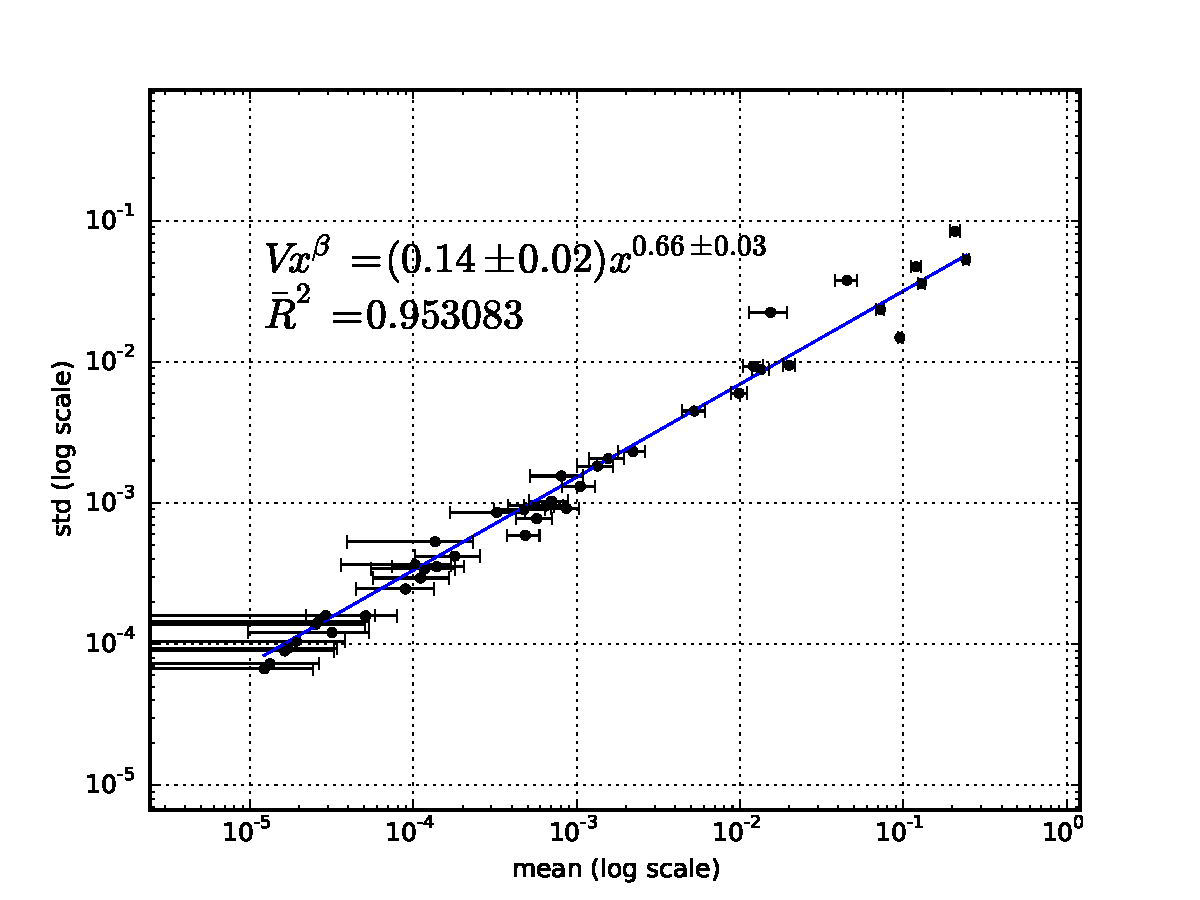
\includegraphics[width=0.8\textwidth]{results/fits/IBS_h_A_amplicons_family_stdVSmean_xWboot_LOG.pdf}
	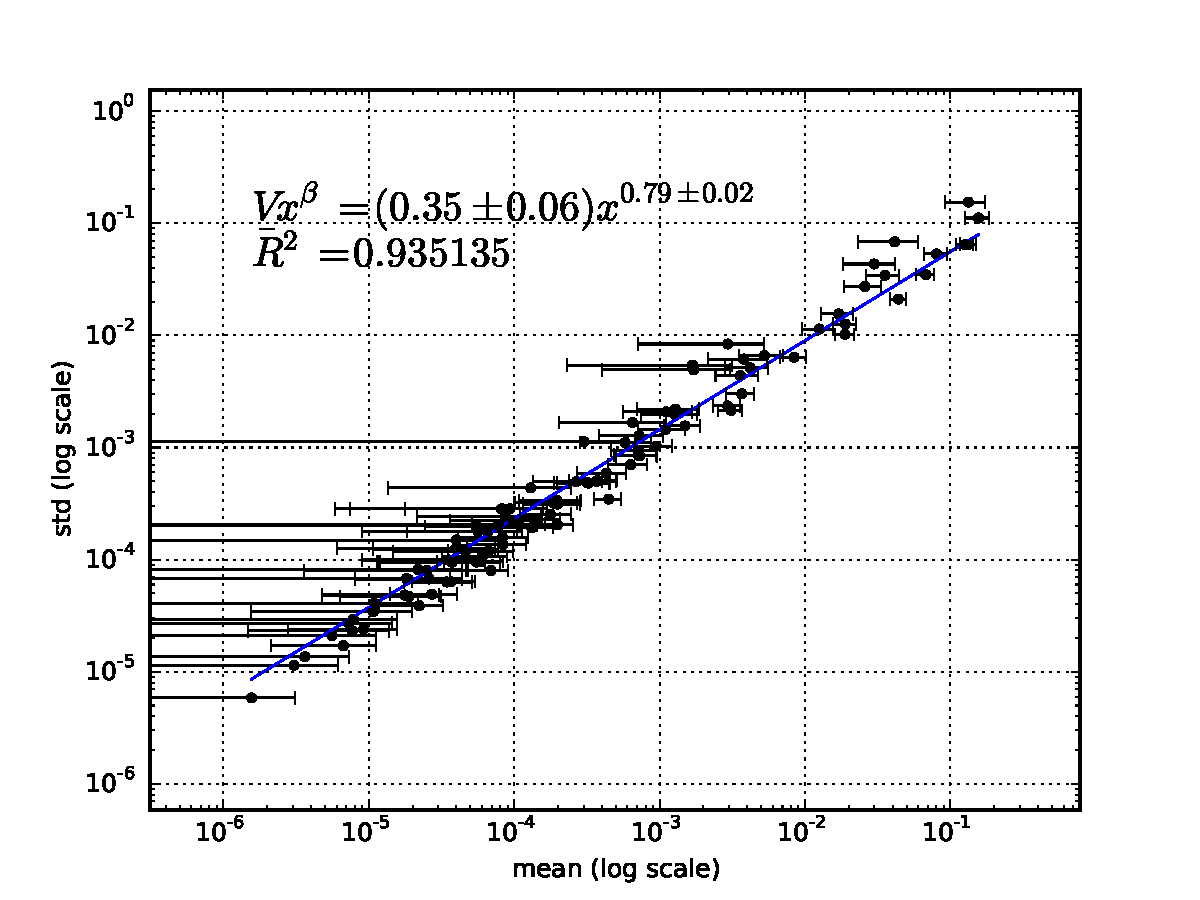
\includegraphics[width=0.8\textwidth]{results/fits/IBS_P2_Metatranscriptores_stdVSmean_xWboot_LOG.pdf}
	\caption{X-weighted power-law fits of the standard deviations (std) versus the mean values for each bacterial genus monitored in time. We show the fit for samples from a healthy subject (top) and from a subject diagnosed with irritable bowel syndrome (bottom), studied in our lab \cite{IBS}. Taylor's power law seems to be ubiquitous, spanning to six orders of magnitude.}
	\label{fig:main1}
\end{figure}

Taylor parameters describing the temporal variability of the gut microbiome in our sampled individuals are shown in Supplementary Tables S1 to S6. Our results hint at an ubiquitous behavior. On the first hand, the variability (which corresponds to the maximum amplitude of fluctuations) is large, which suggests resilient capacity of the microbiota. On the other hand, the scaling index is always smaller than one, which means that more abundant taxa are less volatile than less abundant ones. In addition, Taylor parameters for the microbiome of healthy individuals in different studies are compatible within estimated errors. This enables us to define an area in the Taylor parameter space that we called the \emph{healthy zone}. 

In order to jointly visualize and compare the results of individuals from different studies\cite{IBS,moving,antibiotic,LEA,kwashiorkor,diet}, their Taylor parameters have been standardized, where standardization means that each parameter is subtracted by the mean value and divided by the standard deviation (std) of the group of healthy individuals for each study (for details of the procedure, please see Standardization subsection in Material and Methods). The healthy zone and the standardized Taylor parameters for individuals whose gut microbiota is altered (i.e., suffering from kwashiorkor, altered diet, antibiotics or IBS) is shown in Figure \ref{fig:main2}. Children developing kwashiorkor show smaller variability than their healthy twins. A meat/fish-based diet increases the variability significantly when compared to a plant-based diet. All other cases presented increased variability, which is particularly severe, and statistically significant at more than 95\% CL, for obese patients grade III on a diet, individuals taking antibiotics or IBS--diagnosed patients. A global property emerges from all worldwide data collected: Taylor parameters characterize the statistical behavior of microbiome changes. Furthermore, we have verified that our conclusions are robust to systematic errors due to taxonomic assignment (see Taxa level selection in Material and Methods).

\begin{figure}
	\centering
	\includegraphics[width=0.9\textwidth]{results/finalplot11.pdf}
	\caption{Taylor's law parameter space. We have compiled here all the data studied in this work. The coloured circle corresponds to 68\% confidence level (CL) region of healthy individuals in the Taylor parameter space, while dashed line delimites the 98\% CL region. Points with errors place each individual gut microbiome in the Taylor space. Note that the parameters have been standardized (standard deviation units) to the healthy group in each study for demonstrative and comparative purposes.}
	\label{fig:main2}
\end{figure}

Taylor's power law has been explained in terms of various effects, all without general consensus. It can be shown to have its origin in a mathematical convergence similar to the central limit theorem, so virtually any statistical model designed to produce a Taylor law converge to a Tweedie distribution\cite{stat}, providing a mechanistic explanation based on the statistical theory of errors\cite{convergence1,convergence2,convergence3}. To unveil the generic mechanisms that drive different scenarios in the $\beta$--$V$ space, we model the system by assuming that taxon relative abundance follows a Langevin equation with, on the one hand, a deterministic term that captures the fitness of each taxon and, on the other hand, a randomness term associated with Gaussian random noise\cite{ranking}. Both terms are modeled by power laws, with coefficients that can be interpreted as the taxon fitness $F_i$ and the variability $V$ (see Model under Material and Methods). In this model, when $V$ is sufficiently low, abundances are stable in time. Differences in variability $V$ can induce a noise-induced phase transition in relative abundances of taxa. The temporal evolution of the probability of a taxon having abundance $x_i$ given its fitness is governed by the Fokker--Planck equation. The results of solving this equation show that the stability is best captured by a phase space determined by fitness $F$ and amplitude of fluctuations $V$ (see Figure \ref{fig:main3}). 

\begin{figure}
	\centering
	\vspace*{-5mm} % Corrects overbox of the figures
	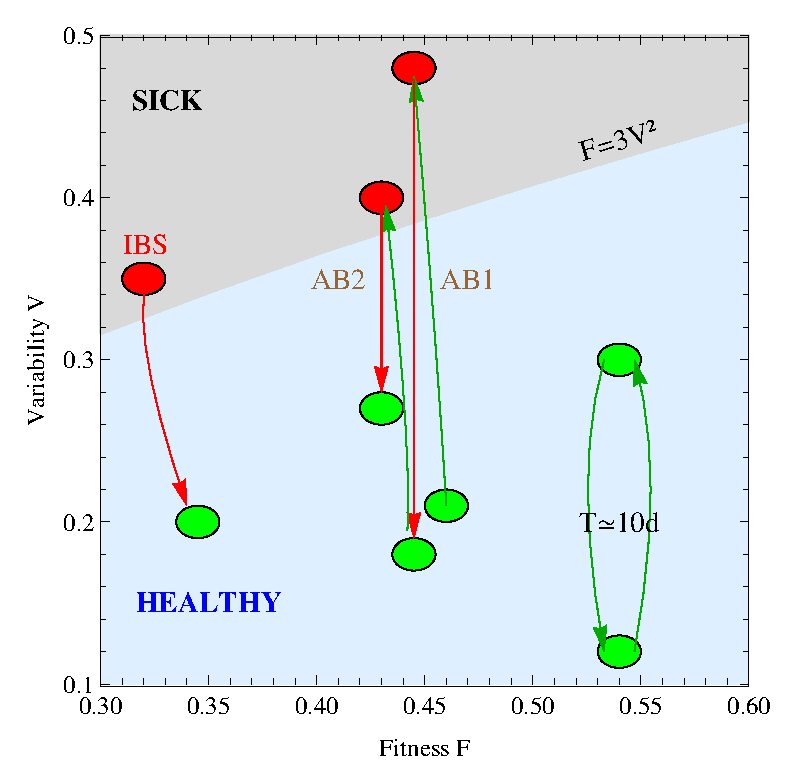
\includegraphics[width=0.8\textwidth]{results/finalPlot33_new.pdf}
	\caption{Microbiota states can be placed in the phase space $F$--$V$. The light blue shaded region corresponds to the stable phase, while the grey shaded region is the unstable phase (the phase transition line is calculated for  $\alpha$ = $\beta$ = 0.75). We place healthy individuals (green) and individuals whose gut microbiota is threatened (antibiotics, IBS) in the phase space fitness--variability. Gut microbiota of healthy individuals over a long term span show a quasi--periodical variability (central period is ten days). We show that taking antibiotics (AB1 and AB2 correspond to first and second treatment respectively) induces a phase transition in the gut microbiota, which impacts its future changes. We also show an IBS--diagnosed patient transiting from the unstable to the stable phase.}
	\label{fig:main3}
\end{figure}

The model predicts two phases for the gut microbiome: a stable phase with large variability that permits some changes in the relative abundances of taxa; and an unstable phase with larger variability, above the phase transition, where the order of abundant taxa varies significantly with time. The microbiome of all healthy individuals was found to be in the stable phase, while the microbiome of several other individuals was shown to be in the unstable phase. In particular, individuals taking antibiotics and IBS--diagnosed patient P2 had the most severe symptoms. In this phase diagram, each microbiota state is represented by a point at its measured variability $V$ and inferred fitness $F$. The model predicts high average fitness for all taxa, i.e., taxa are narrowly distributed in F. The fitness parameter has been chosen with different values for demonstrative purposes. Fitness is larger for the healthiest subjects and smaller for the IBS--diagnosed patients.

%%%
\subsection*{Rank stability of the taxa} 

\def \RSItable {
\scriptsize
	\begin{tabular}{cccr}
	\multicolumn{4}{c}{Colour code for the RSI percentage column} \\
    \hline
    Case  &  Condition  &  Colour  &  Description \\
    \hline
    1  &  $1\ge{\rm RSI}>0.99$  & \textcolor{blue}{blue} & constant rank \\ 
    2  &  $0.99\ge{\rm RSI}>0.90$  &  \textcolor{green}{green}  & highly stable rank \\
    3  &  $0.90\ge{\rm RSI}>0.75$  &  \textcolor{orange}{orange} & moderately stable rank \\
    4  &  $0.75\ge{\rm RSI}>0.25$  &  \textcolor{red}{red} & unstable rank \\
    5  &  $0.25\ge{\rm RSI}\ge0$  &  \bfseries{black} & very unstable rank \\
    \hline
    \end{tabular}	
}

The rank dynamics and stability plots in Figure \ref{fig:corrank_IBS_A} and \ref{fig:corrank_IBS_P2} show the variation in the rank with time for the most dominant taxa and their calculated Rank Stability Index (RSI, as discussed in Material and Methods) for the taxa of a healthy subject (individual \emph{A}, Figure \ref{fig:corrank_IBS_A}) and from a subject diagnosed with IBS (patient \emph{P2}, Figure \ref{fig:corrank_IBS_P2}) of the IBS study\cite{IBS}. The taxa are listed ordered by the accumulated frequency along the time series, so y-axis is an overall dominance axis for each sample set. Generally speaking, we observe that the most dominant taxa are the most rank stable. 

\begin{figure}
	\centering
	%\vspace*{-10mm} % Corrects overbox of the figures
	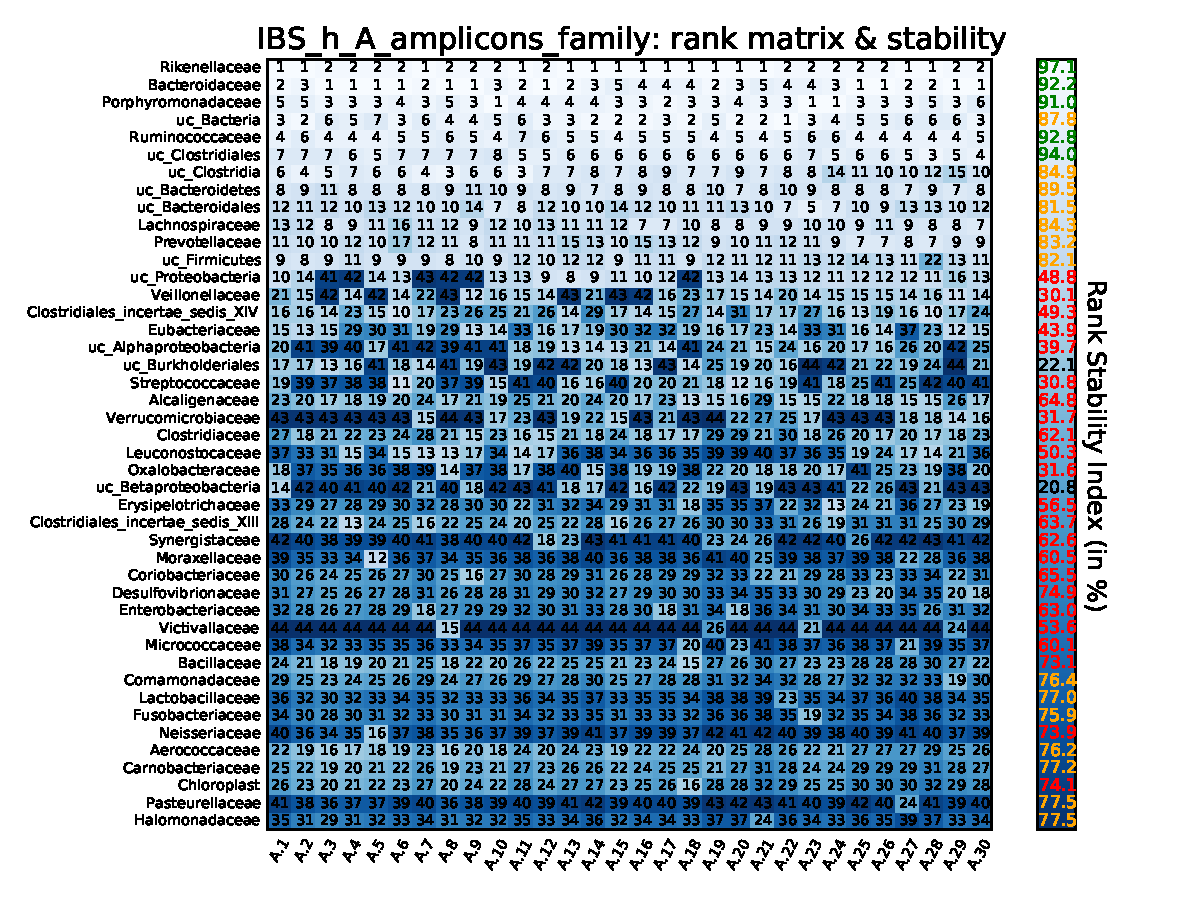
\includegraphics[width=0.99\textwidth]{results/corrank/IBS_h_A_amplicons_family_Rank.pdf}
	\RSItable	
	\caption{Rank variation throughout time for the most dominant elements (taxa) and their calculated Rank Stability Index (as shown in Material and Methods) for samples from a healthy subject studied in our lab\cite{IBS}.}
	\label{fig:corrank_IBS_A}
\end{figure}

\begin{figure}
	\centering
	%\vspace*{-10mm} % Corrects overbox of the figures
	\hspace*{-4.5mm}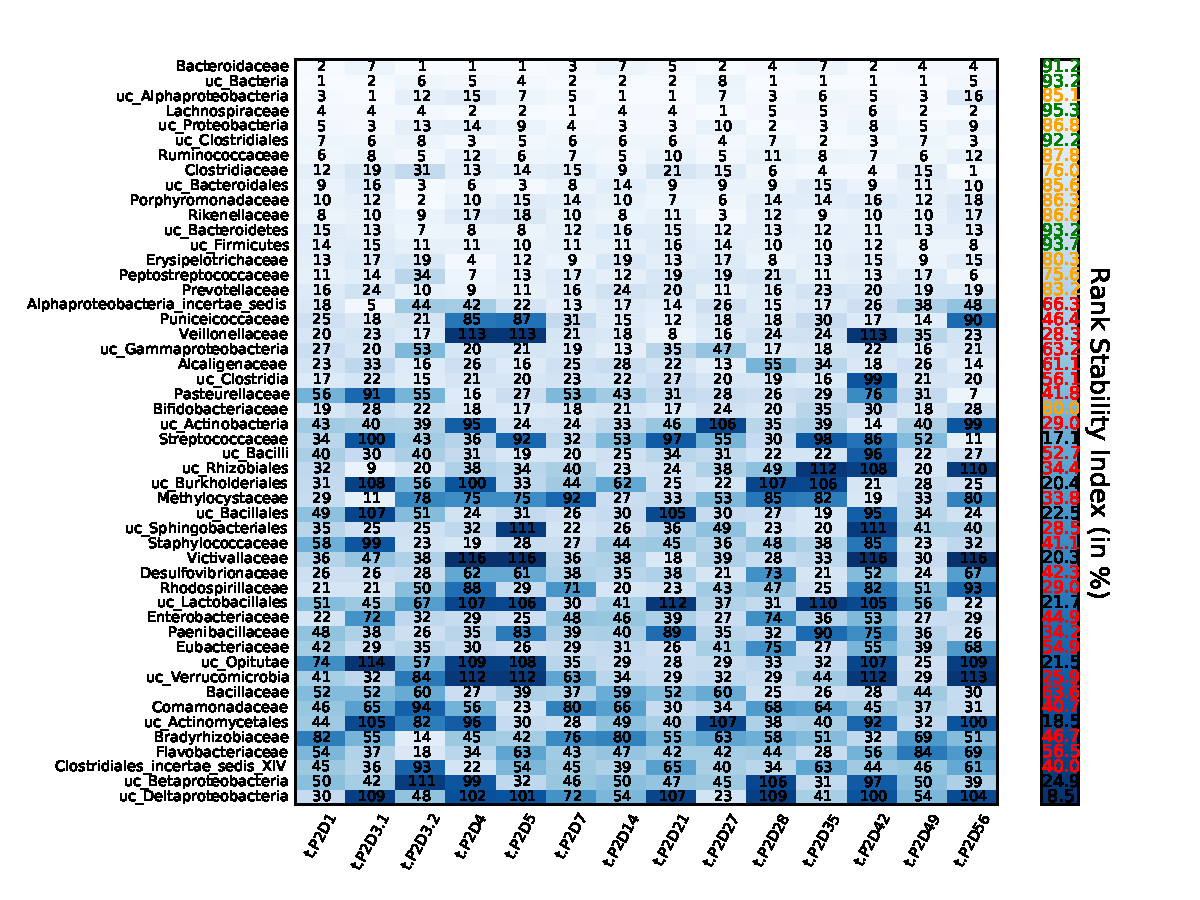
\includegraphics[width=0.99\textwidth]{results/corrank/IBS_P2_Metatranscriptores_Rank.pdf}
	\RSItable
	\caption{Rank variation throughout time for the most dominant elements (taxa) and their calculated Rank Stability Index for samples from a subject diagnosed with irritable bowel syndrome studied in our lab\cite{IBS}.}
	\label{fig:corrank_IBS_P2}
\end{figure}

Nevertheless, in the particular case of the healthy individual in Figure \ref{fig:corrank_IBS_A}, \emph{Burkholderiales} and \emph{Betaproteobacteria} (taxa ordered as 18th and 25th in the dominance axis) show comparatively very low rank stability regarding similar dominant taxa while, on the other hand, \emph{Comamonadaceae}, \emph{Lactobacillaceae}, \emph{Fusobacteriaceae}, \emph{Aerococcaceae} and \emph{Carnobacteriaceae} show higher stability than other more dominant taxa, forming a kind of \emph{rank stability island} for medium-ranked taxa around position 40 in the dominance axis, and thus colored in orange, following the color criteria shown in the table included in Figure \ref{fig:corrank_IBS_A}, since they show a moderately stable RSI.

In the IBS diagnosed patient of Figure \ref{fig:corrank_IBS_P2}, beyond the differences in dominance for the particular taxa, we still observe that the most dominant are the most rank stable. However, as opposed to the healthy individual results, far from presenting a \emph{rank stability island}, the medium-ranked taxa are very rank unstable, mostly due to transient (often one or two consecutive samples) but deep drops in their relative abundance, which are usually happening more than twice along the time series. That is, for instance, the case of \emph{Sphingobacteriales} with two non-consecutive samples dropping to 111th rank position. In other cases, the high rank instability comes from a rank fluctuation over all the time series, as for \emph{Streptococcaceae} and \emph{Burkholderiales}, which are ranking 26th and 29th respectively in the overall dominance axis but show very low RSI, and thus colored in black attending to the color criteria shown in the table included in Figure \ref{fig:corrank_IBS_P2}.

We found the presence of such of \emph{rank stability island} for medium-ranked taxa in the other healthy subjects (\emph{B} and \emph{C}) of the IBS study\cite{IBS} together with its total absence for the other IBS diagnosed patient (patient \emph{P1}), which also presents very high rank instability in its medium-ranked taxa.


%%%
\subsection*{Time dependence of model parameters}

Finally, we have studied the time dependence of the variability $V$ and power law index $\beta$ (see Model under Material and Methods) by using a sliding window approach. The total number of time points are divided in subsets of five points, where the next subset is defined by adding the next time sampling and by eliminating the earliest one. Both parameters were calculated for each subset against the average time lapse. Figure \ref{fig:tempevo1} shows the variability  $V$ as a function of time for the largest sampling: two individuals in the Caporaso's study\cite{moving} corresponding to the gut microbiota of a male (upper plot) and a female (lower plot). Figure \ref{fig:tempevo2} shows the time evolution of $V$ for patient P2 of the IBS study\cite{IBS} (upper plot) and patient D in the antibiotics study\cite{antibiotic} (lower plot). Both samples shows changes in the variability V with quasi--periodic behavior peaked at about 10 days. Variability grows more for the gut microbiota of the male and share a minimal value around 0.1 with the gut microbiota of the female. The variability of the gut microbiota of P2 decreases from above 0.3 to below 0.2, showing a slow tendency to increase the order of the system.  Antibiotic intake leaks to a quick increase of variability which lasts for a few days to recover ordering. The second antibiotic treatment shows some memory (lower increase of variability) with a slower recovery.

\begin{figure}
	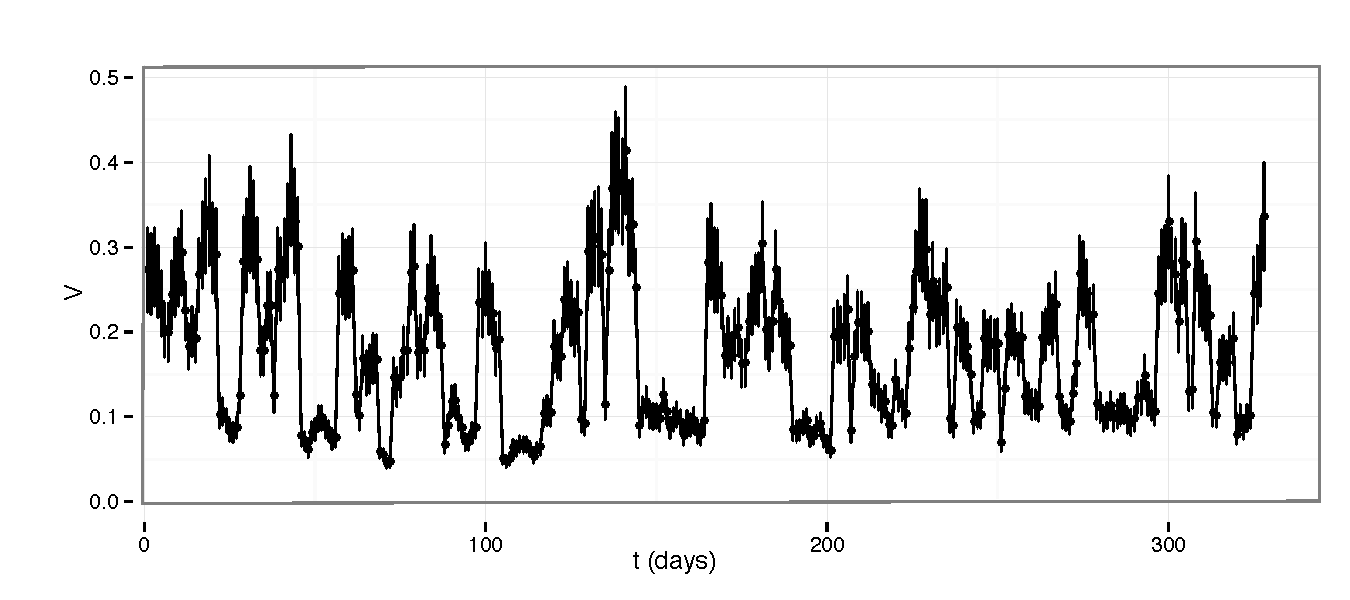
\includegraphics[width=1.0\textwidth]{results/sliwin/male_mov.pdf}
	\hspace*{3mm}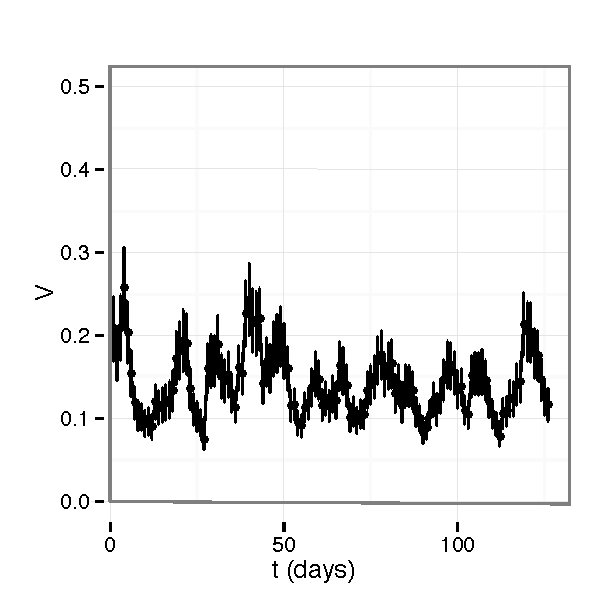
\includegraphics[width=0.448\textwidth]{results/sliwin/female_mov.pdf}
\caption{$V$ as a function of time for the two individuals in the Caporaso's study\cite{moving}: samples of gut microbiome of a male (upper plot) and a female (lower plot).}
\label{fig:tempevo1}
\end{figure}

\begin{figure}
	\centering 
 	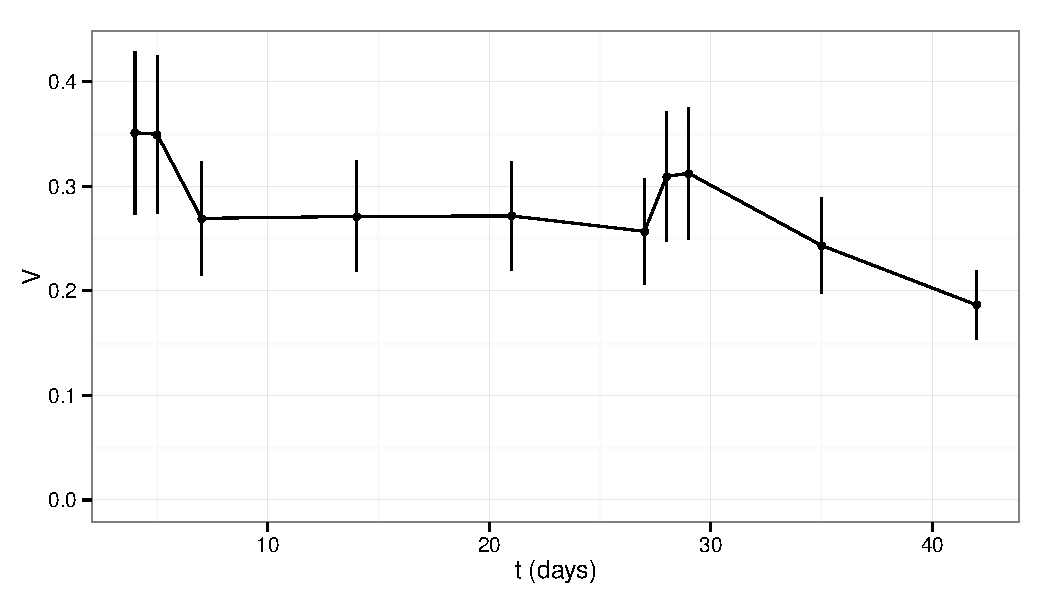
\includegraphics[width=0.8\textwidth]{results/sliwin/patP2_IBS.pdf}
  	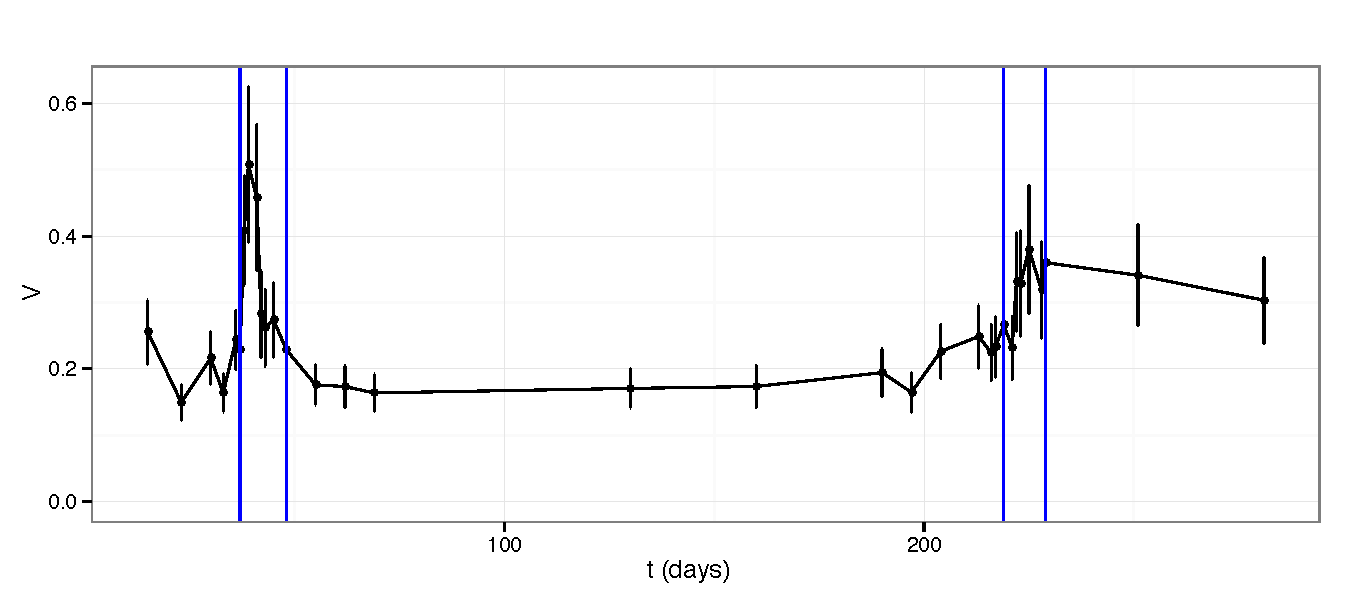
\includegraphics[width=1.0\textwidth]{results/sliwin/patD_antibio.pdf} 
\caption{$V$ as a function of time for patient P2 of the IBS study\cite{IBS} (upper plot) and patient D in the antibiotics study\cite{antibiotic} (lower plot). The blue vertical lines in the lower plot are showing the periods of antibiotic treatment.}
\label{fig:tempevo2}
\end{figure}

\clearpage
%%% Discussion
\section*{Discussion}
One of the mains features of this work is to have shown that, independently of its condition, the microbiota follows the Taylor's law. We have seen that the value of the scaling index in each case is always less than the unity (using standard deviation as the measurement for dispersion), which is informing us about the community structure. This means that, in relative terms, the most abundant elements in the population are less volatile to perturbations than the less abundant ones. The explanation for this universal pattern is not clear although some hypothesis have been tested in other studies, as the presence of negative interactions in the population \cite{kilpatrick}, or the demonstration that it may depend on reproductive correlation \cite{ballantyne}. Nevertheless, none of these explanations are enough when we are talking about microbiota as the reproduction term is diffuse, the interactions between its components are not only based on competition \cite{joao, mehta, bucci} and that even that kind of negative interaction may not effectively yield in values less than the unity when referring to a bacterial species \cite{ramslayer}. Anyhow, the values obtained in all cases are very similar among them, which could be suggesting that the community structure is preserved throughout the different scenarios that we have studied.

The second parameter is informing about the noise and can be directly related with the variability or the fluctuation amplitude of the population over time. It is a direct estimator of the stability of the system under study. As we showed above, the healthy subset of each study have lower variability than the non-healthy subset when dealing with adult individuals. Interestingly, the variability parameter was higher in the healthy subset for the study of the discordant twins suffering from kwashiorkor disease \cite{kwashiorkor}. Taking into account that the infant microbiota is evolving toward a definite, adult state \cite{koenig}, it means that the temporal variability would be greater than in a adult who has reached a stability in his gut microbiota, while our results could be directing in the possibility that this variability is necessary in order to reach that adult state  \todo{<-review the wording of the whole sentence}. Furthermore, as we wanted to see how this variability behaved over time, we calculated the evolution of this parameter for the samples which had enough time sampling. As can be seen in Figure \ref{fig:tempevo1}, the variability of the microbiota has some fluctuations over time. It is interesting to note in Figure \ref{fig:tempevo2} how this parameter can capture the two antibiotic intakes in one of the patients from the study of Dethlefsen and Relman \cite{antibiotic}, especially that it seems to be some resilience process in the microbiota due to the lower variability increase in the second antibiotic intake.  

The primary hypothesis of this work is that, in adults, having a healthy microbiota means that population is stable in time and does not have huge flips or jumps into another states. In order to use the valuable information which gives us the empirical law of Taylor's work, we propose the use of Langevin equation to model how the ranking stability evolves in time. While we can measure directly the component of the noise of the system as their variability, the other main term needs to be inferred from the model. This term, which we have named as 'fitness', is the one that gives the ability to the system to be stable to potential perturbations. In ecological terms, this could mean the nature of interactions that are present among the bacteria, between bacteria and other minority populations as fungi or archaea, between bacteria and the viral component in the microbiota, and the interactions between host and the whole microbiota. Being this a first step to model the temporal stability of the microbiota and due to its complicated nature, we have calculated the fitness term using the Fluctuation Dissipation Theorem as a first approximation\cite{FD}. Thus, the fitness of the microbiota still remains to be modelled in future works in order to make the model more accurate and with a higher predictive power. 

By solving the Langevin differential equation, we can obtain a phase diagram where each microbiota sample can be placed according to its fitness and variability in one of two phases according to the ranking stability of the system. As we can see in the phase-space in Figure \ref{fig:main3}, we are showing three different conditions that could happen. First, we can have a healthy microbiota which could have some fluctuations as showed by one of the subjects of Caporasso et al study \cite{moving}. Because the fitness of this cases will be high enough, the temporal variability will not place the microbiota in the unstable phase of the diagram. Second, we have a subject from the study of Dethlefsen and Relman \cite{antibiotic} which is perturbed twice by an antibiotic intake. His microbiota is altered enough to lose its stability, and hence be placed in the unstable part. So located, it is more sensible to potential perturbations as, for example, opportunist infections. Third and last condition, the subject is already in the unstable phase due to some healthy issue as IBS. This can be observed in one of the patients from Durban et al study \cite{IBS}. In addition, it was shown that this subject improved its healthy status in the time when the experiment was done, implying that his microbiota also recovered the lost stability. 

Specifically, the analysis of the rank stability of the samples of healthy and IBS diagnosed patients studied in our lab\cite{IBS}, suggests that the presence of \emph{rank stability islands} among medium-ranked taxa is a interesting feature. The higher stability of these taxa goes against the global meaning of the scaling index. Interestingly, that stability disappears when we look at the IBS patients. One could ask if these taxa are key players in the phase transition of the microbiota, of if they are more susceptible to perturbations than the most abundant. The types of interactions that could be sustaining this particular behavior are not clear, as these non-abundant taxa are not usually included in dynamical studies in order to get the community matrix. Further experiments and data analysis is needed to clarify if this is not a unique event, or it is a widespread feature of stable microbiotas. 

However, we have to be aware that the hypothesis above is too simplistic to be directly related with reality. It has been demonstrated that the situation is more complex than the outlook provided separating healthy people from non-healthy people just by compositional terms, as Moya and Ferrer underline in their recent review \cite{Moya_trends}. There are several different feasible scenarios in which we can consider the microbiota as stable independently of their compositional evolution over time. For example, depending on their ability to recover the initial composition (resilience), or whether it can recover the original function despite the composition (functional redundancy). What we have shown in this work could be explained as the transitions of a stable microbiota into a dysbiosis state.  

As a first step toward understanding the microbiota stability, the model presents some limitations and there is still work to do. From the biological perspective, many questions arise from this work. We have observed the same pattern in Taylor's parameters in all the different conditions we have studied, but a pertinent question is whether it is really a universal feature in the huge diversity of microbial niches. Furthermore, another relevant question is which mechanisms are involved in maintaining the population structure. The nature of the interactions among the elements of the community is surely of great importance in this matter, and it is related to the fitness of the community as has been commented above. How we should address the community fitness is not clear, but works as Tikhonov's \cite{tikhonov} could help us to aim at the correct direction toward unraveling the complexity of the microbiota.
\clearpage    
%%% Material & Methods
\section*{Materials and Methods}
We summarize our dataset in ST1-6 (Tables 1-6 in suplemental material). The bacteria and archaea taxonomic assignations were obtained by analysing 16S rRNA sequences, which were clustered into operational taxonomic units (OTUs) sharing 97 \% sequence identity using QIIME\cite{QIIME}. WGS data\cite{kwashiorkor} were analysed and assigned at strain level by the Livermore Metagenomic Analysis Toolkit (LMAT)\cite{LMAT}, according to their default quality threshold. Genus, with best balance between error assignment and number of taxa, was chosen as our reference taxonomic level. We have verified that our conclusions are not significantly affected by selecting family or species as the reference taxonomic level (see Figure 1 in supplemental material).

\todo{Specify, in each study treated, the nature of the samples (conditions, timespan between timepoints, subjects). Specify, and it is very important, what we consider ?healthy? in each study (for example: pre-antibiotics is healthy)}

%%%
\subsection*{Model} \label{sec:model}

We model the microbial abundances across time along the lines of Blumm \textit{et al.}\cite{ranking}. The dynamics of taxon relative abundances is described by the Langevin equation:
\begin{linenomath}
\begin{equation}
\dot{x_i} = F_i \cdot x_i^\alpha + V \cdot x_i^\beta \xi_i(t) - \phi(t) \cdot x_i,
\end{equation}
\end{linenomath}
where F$_i$ captures the fitness of the taxon i, V corresponds to the noise amplitude and $\xi_i$(t) is a Gaussian random noise with zero mean  $<\xi_i(t)>$ = 0 and variance uncorrelated in time, $<\xi_i(t) \xi_i(t')>$ =  $\delta(t'-t)$, . The function $\phi(t)$ ensures the normalization at all times, $\sum x_i(t) = 1$, and corresponds to $\phi(t) = \sum F_i x_i^\alpha + \sum V x_i^\beta \xi_i(t)$.
The temporal evolution of the probability that a taxon i has a relative abundance $x_i(t)$, P(x$_i$,t), is determined by the Fokker-Planck equation:
\begin{linenomath}
\begin{equation}
\frac{\partial P}{\partial t} = - \frac{\partial}{\partial x_i}  [(F_i \cdot x_i^\alpha - \phi(t) \cdot x_i ) \cdot P]+ \frac{1}{2} \frac{\partial^2}{\partial x_i^2} (V^2 \cdot x_i^{2\beta}\cdot P).
\end{equation}
\end{linenomath}
The microbiota evolves towards a steady-state with a time-independent probability depending on the values of $\alpha$, $\beta$, F$_i$ and V. For $\alpha<1$ (otherwise, systems are always unstable), the steady-state probability may be localized in a region around a preferred value or broadly distributed over a wide range, depending on whether the fitness F$_i$  dominates or is overwhelmed by the noise amplitude V. The steady-state solution of the Fokker-Planck equation is given by:
\begin{eqnarray}
P_0 (x_i) &=& C_{ne}(\alpha,\beta,F_i,V)  \cdot x_i^{-2\beta}  \cdot \exp\Big[\frac{2F_i}{V^2}\frac{x_i^{1+\alpha-2\beta}}{1+\alpha-2\beta}-\frac{\phi_0}{V^2}\frac{x_i^{2-2\beta}}{1-\beta}\Big] \quad \textrm{if} \quad  2\beta \ne 1+\alpha, \notag \\
P_0 (x_i) &=& C_e(\alpha,\beta,F_i,V)  \cdot x_i^{\frac{2F_i}{V^2} -2\beta}  \cdot \exp\Big[\frac{\phi_0}{V^2}\frac{x_i^{2-2\beta}}{1-\beta}\Big] \quad \textrm{if} \quad  2\beta = 1+\alpha,
\notag
\end{eqnarray}
where $\phi_0 = (\sum_i F_i^{1/(1-\alpha)})^{1-\alpha}$ and C$_{ne}$ and C$_{e}$ are integrals that should be solved numerically for the parameters of interest. The ordered phase happens when the solution has a maximum in the physical interval ($0<x_i<1$). For larger V, the transition to a disordered phase happens when the maximum shifts to the unphysical region $x_i<0$, which sets the phase transition region V($\alpha,\beta,F_i$). The phase transition region can be calculated analytically in particular cases:
\begin{eqnarray}
F_i^2 &=& 4 \beta \phi_0 V^2\quad \textrm{if} \quad  \beta = \alpha \neq 1, \notag \\
F_i &=& \beta V^2\quad \textrm{if} \quad  2\beta = 1+\alpha,
\notag
\end{eqnarray}
where the first case, simplifies to $F= 3 V^2$ if $\beta = 0.75$ and the fitness of this taxon dominates in $\phi_0$. 
In many physical systems (Brownian motion is the classical example), the two terms of the Langevin equation are related.  The \emph{fluctuation--dissipation theorem} states a general relationship between the response to an external disturbance and the internal fluctuations of the system\cite{FD}. The theorem can be used as the basic formula to derive the fitness from the analysis of fluctuations 
of the microbiota, assuming that it is in equilibrium (the ordered phase).  

\todo{Explain better the fluctuation-dissipation theorem}


%%%
\subsection*{Selection and Methods}

\subsubsection*{Sample selection}
We have chosen studies about relevant pathologies containing metagenomic sequencing time data series of bacterial populations from humans in different healthy and non-healthy states. We have selected only those individuals who had three or more time points of data available in databases. Metadata of each study is provided in Supplementary Tables \ref{tab:diet} to \ref{tab:LEA}. All used 16S rRNA gene sequencing except for the study of the discordant kwashiorkor twins\cite{kwashiorkor} (see Supplementary Tables \ref{tab:DH} and \ref{tab:DK}) where shotgun metagenomic sequencing (SMS) and 16S rRNA were used. In the latter case we selected to work with SMS data to show that our method is valid regardless of the source of taxonomic information. Each one of the datasets was treated as follows:

\subsubsection*{16rRNA sequences processing}
Reads from the selected studies were first quality filtered using the FastX toolkit\cite{FASTX}, allowing only those reads which had more than 25 of quality along the 75\% of the complete sequence. 16S rRNA reads were then clustered at 97\% nucleotide sequence identity (97\% ID) into operational taxonomic units (OTUs) using QIIME package software\cite{QIIME} (version 1.8) We followed open reference OTU picking workflow in all cases. The clustering method used was uclust, and the OTUs were matched against Silva database\cite{SILVA} (version 111, July 2012) and were assigned to taxonomy with an uclust-based consensus taxonomy assigner. The parameters used in this step were: similarity 0.97, prefilter percent id 0.6, max accepts 20, max rejects 500. 

\subsubsection*{Metagenomic sequences processing}
Metagenomic shotgun (and 16S too) sequences were analyzed with LMAT (Livermore Metagenomics Analysis Toolkit) software package\cite{LMAT} (version 1.2.4, with Feb'15 release of data base \emph{LMAT-Grand}). LMAT was run using a Bull shared-memory node belonging to the team's HPC (high performance computing) cluster. It is equipped with 32 cores (64 threads available using Intel Hyper-threading technology) as it has 2 Haswell-based Xeons, the E5-2698v3@2.3 GHz, sharing half a tebibyte (0.5 TiB, that is, 512 gibibytes) of DRAM memory. This node is also provided with a card PCIe SSD as NVRAM, the P420m HHHL, with 1.4 TB, and 750000 reading IOPS, 4 KB, achieving 3.3 GB/s, which Micron kindly issued free of charge, as a sample for testing purposes. The computing node was supplied with a RAID-0 (striping) scratch disk area. We used the ``Grand'' database\footnote{In this context, ``Grand'' refers to a huge database that contains k-mers from all viral, prokaryote, fungal and protist genomes present in the NCBI database, plus Human reference genome (hg19), plus GenBank Human, plus the 1000 Human Genomes Project (HGP). This represent about 31.75 billion k-mers occupying 457.62 GB.}, release Feb'15, provided by the LMAT team. Previously to any calculation, the full database was loaded in the NVRAM. With this configuration the observed LMAT sustained sequence classification rate was $20\unclassrate$. Finally, it is worth mentioning that a complete set of Python scripts have been developed as back-end and front-end of the LMAT pipeline in order to manage the added complexity of time series analysis. 

\subsubsection*{Taxa level selection}
We selected genus as taxonomic level for the subsequent steps of our work. In order to ensure that, between adjacent taxonomic levels, there were not crucial differences which could still be of relevance after standardization (see Section \ref{sec:stan}), we tested two different data sets. In the former, the antibiotics study\cite{antibiotic} with 16S data, we tested the differences between genus and family levels. The latter dataset tested was the kwashiorkor discordant twins study\cite{kwashiorkor} for both genus and species taxonomic levels. The Supplementary Figures \ref{fig:taxlev1} (overview) and \ref{fig:taxlev2} (detail) plot the comparison between studies (and so, 16S and SMS) and between adjacent taxonomic levels.

\begin{figure} 
  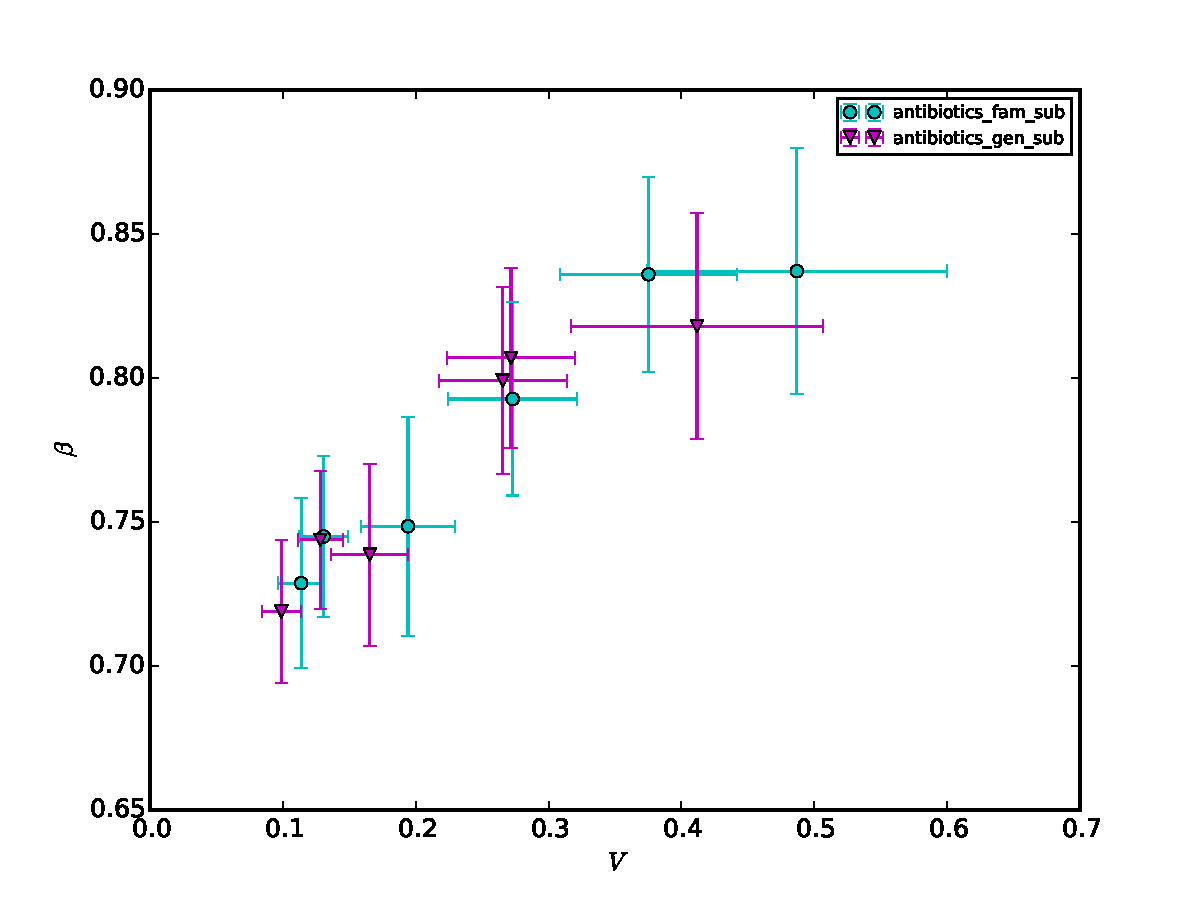
\includegraphics[width=0.5\textwidth]{results/taxalevel/sum_raw_16S.pdf}
  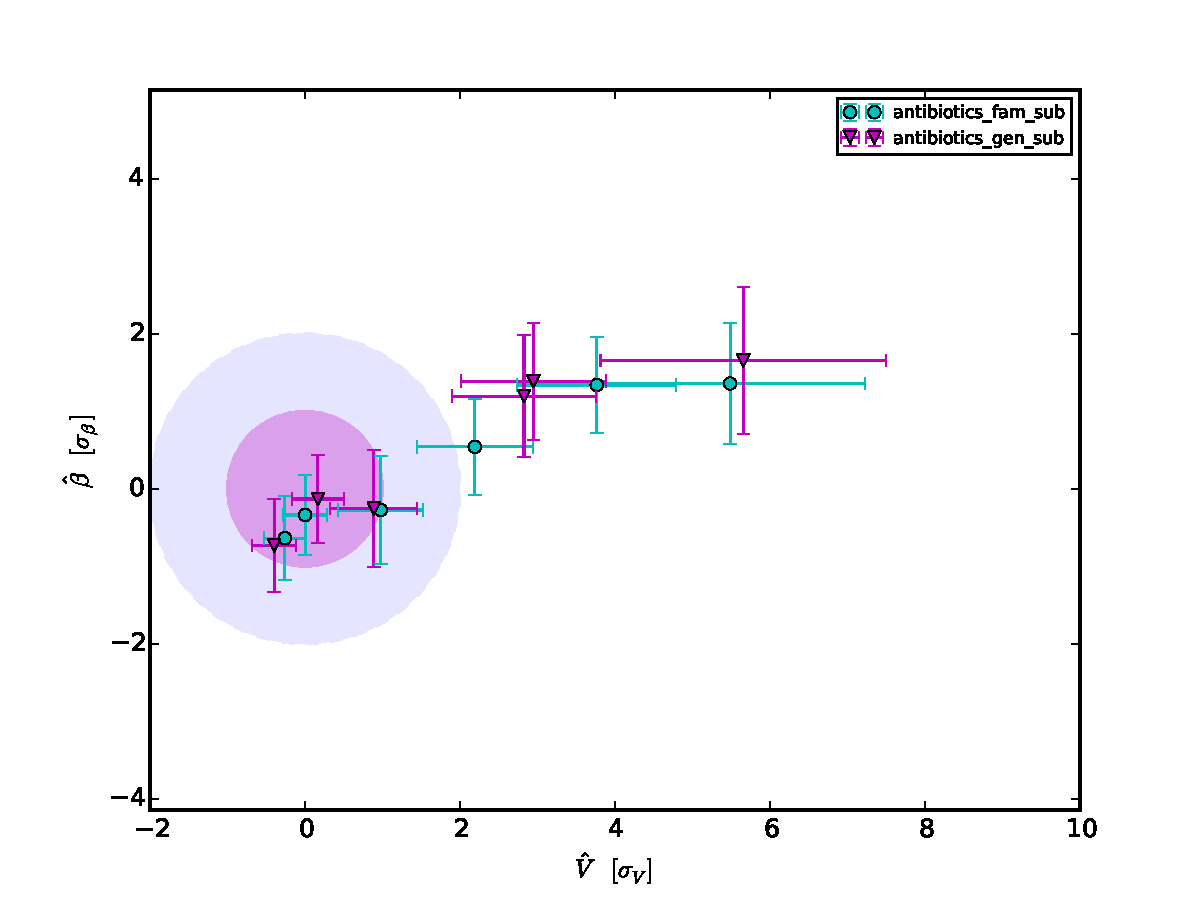
\includegraphics[width=0.5\textwidth]{results/taxalevel/sum_sta_16S.pdf}
  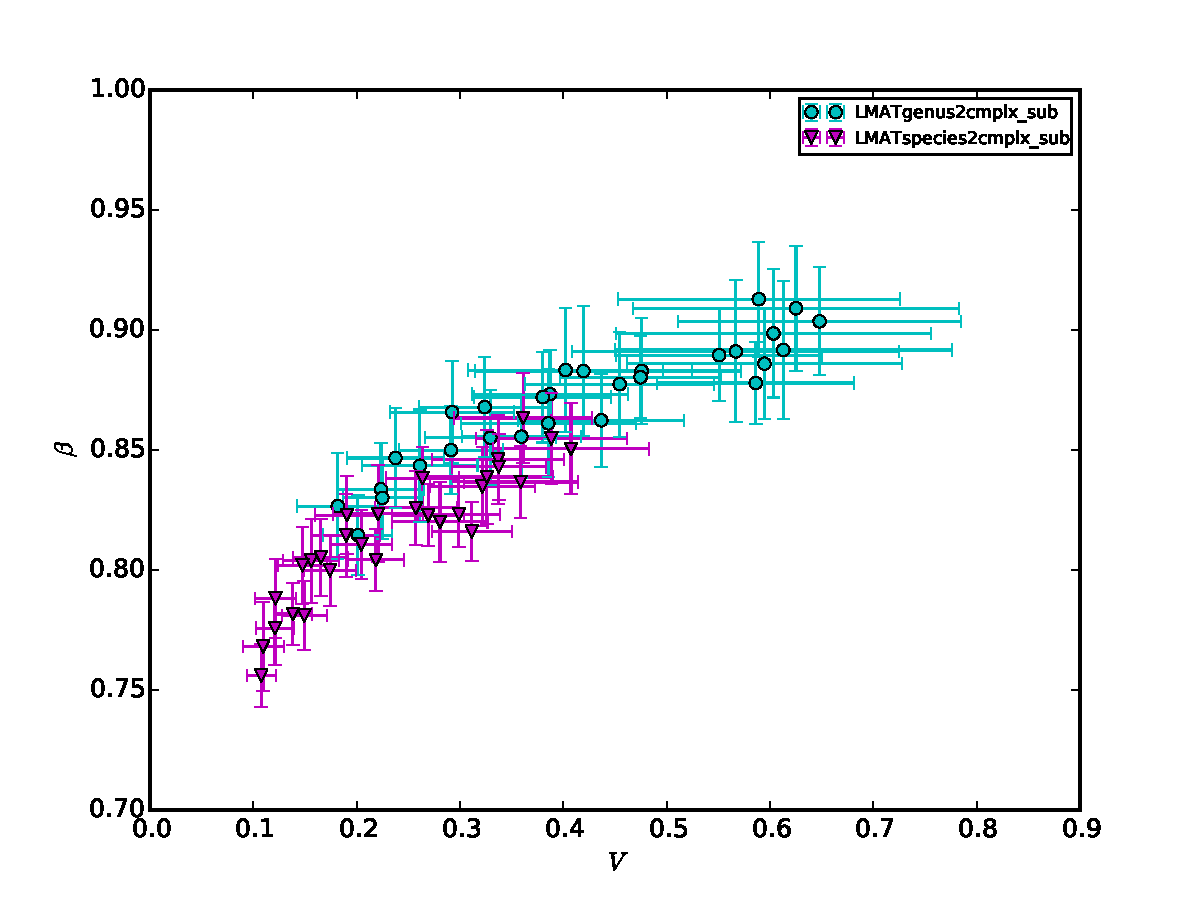
\includegraphics[width=0.5\textwidth]{results/taxalevel/sum_raw_SMS.pdf} 
  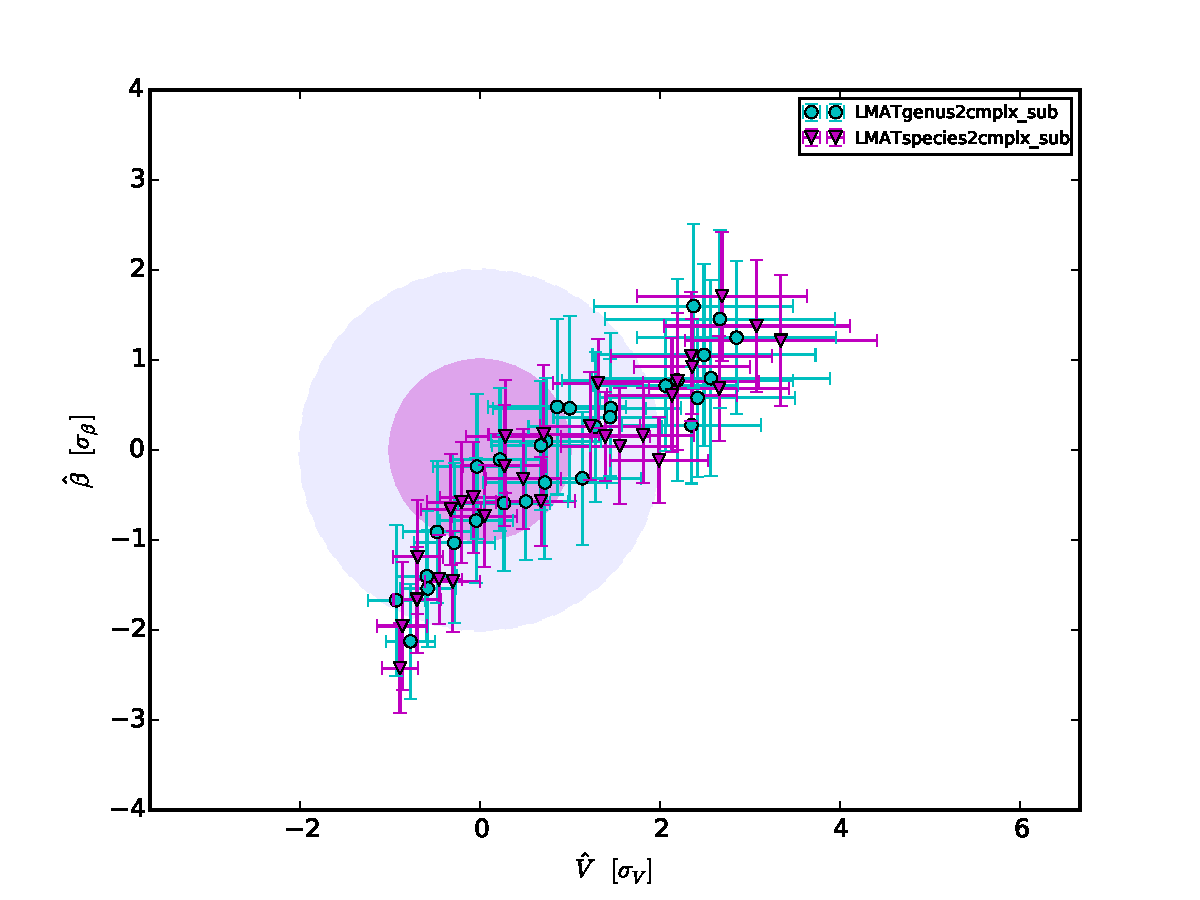
\includegraphics[width=0.5\textwidth]{results/taxalevel/sum_sta_SMS.pdf}
\caption{Overview of comparison of different approaches based on adjacent taxonomic levels using plots in the Taylor-parameters space. For 16S (former row of subfigures), the levels are family vs. genus, whereas for SMS (latter row of subfigures) levels are genus vs. species. The left column shows the raw results and the right column plots the standardized results (see Section \ref{sec:stan})}
\label{fig:taxlev1}
\end{figure}

\begin{figure} 
  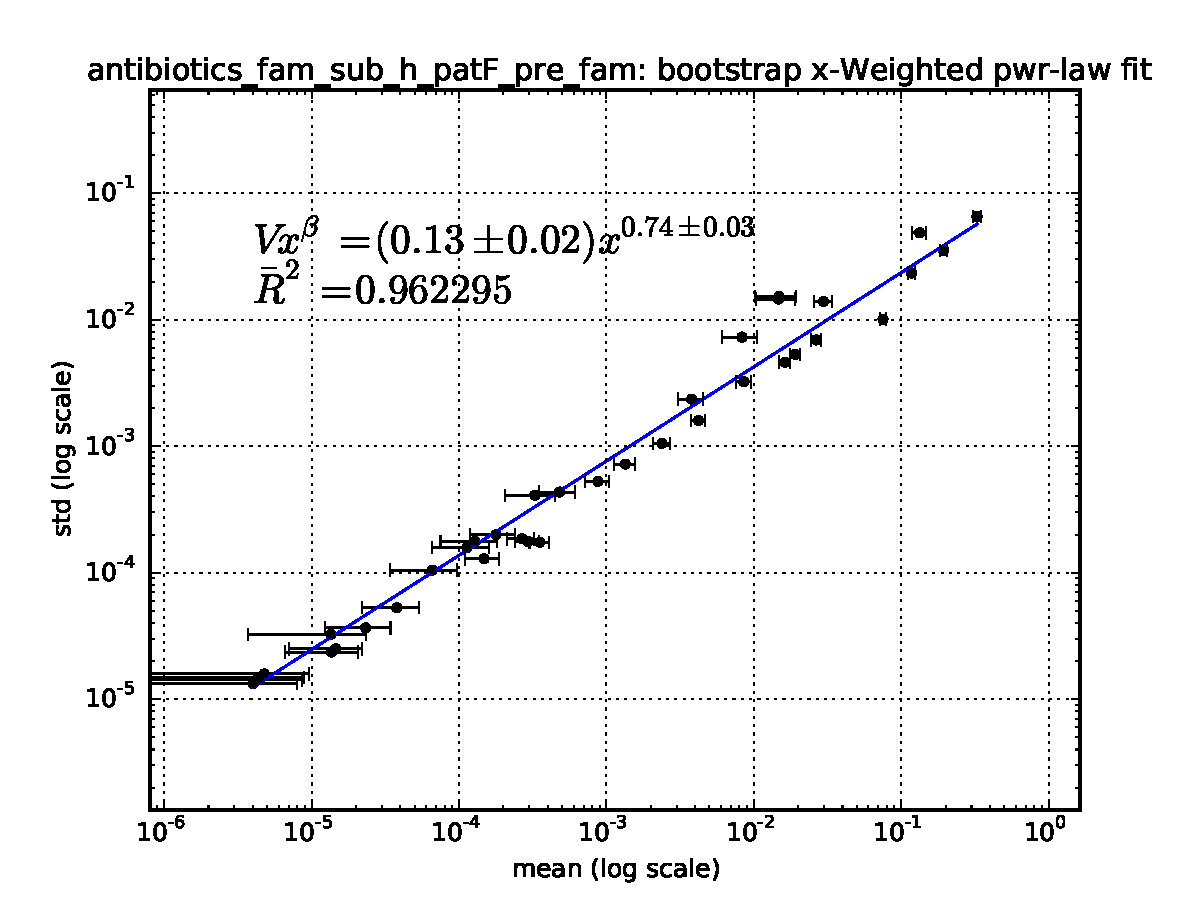
\includegraphics[width=0.5\textwidth]{results/taxalevel/xWb_fam_16S.pdf}
  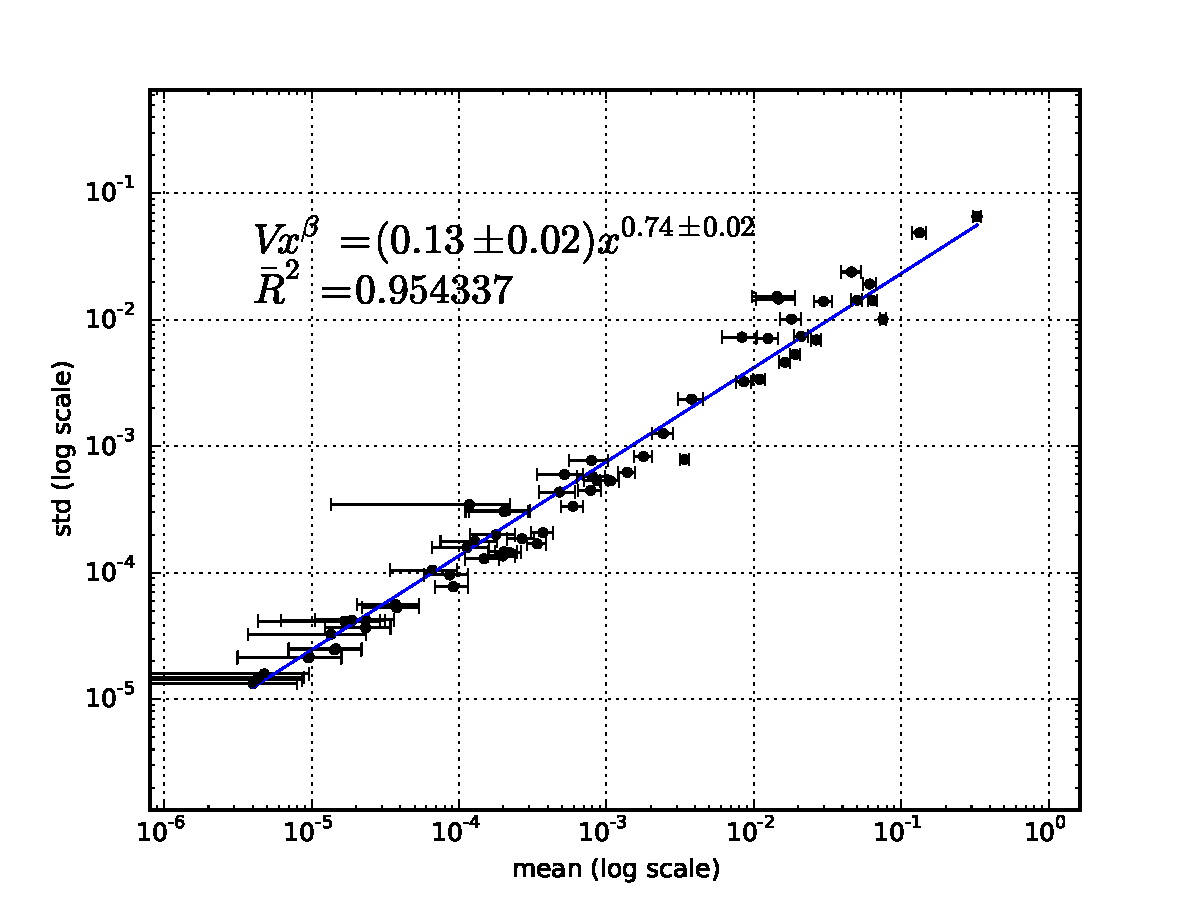
\includegraphics[width=0.5\textwidth]{results/taxalevel/xWb_gen_16S.pdf}
  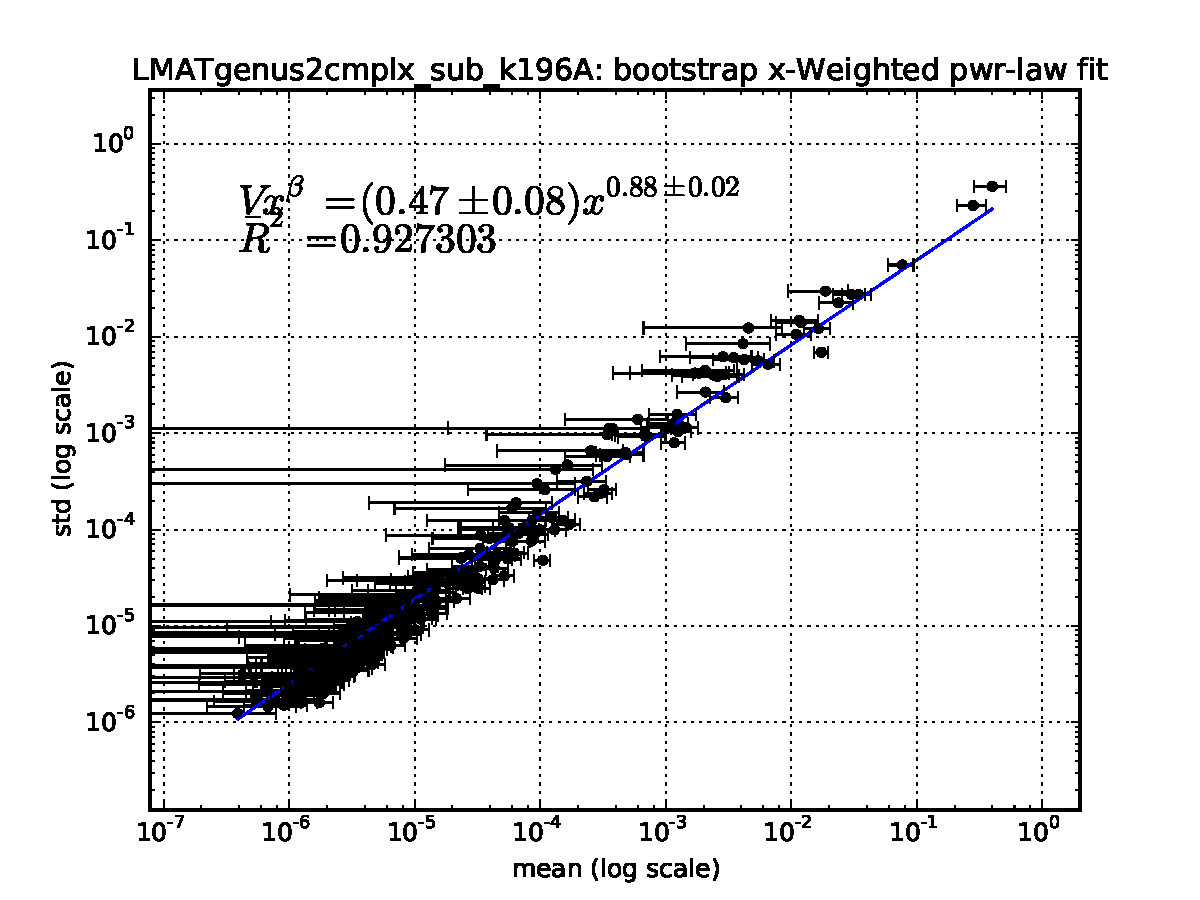
\includegraphics[width=0.5\textwidth]{results/taxalevel/xWb_gen_SMS.pdf}
  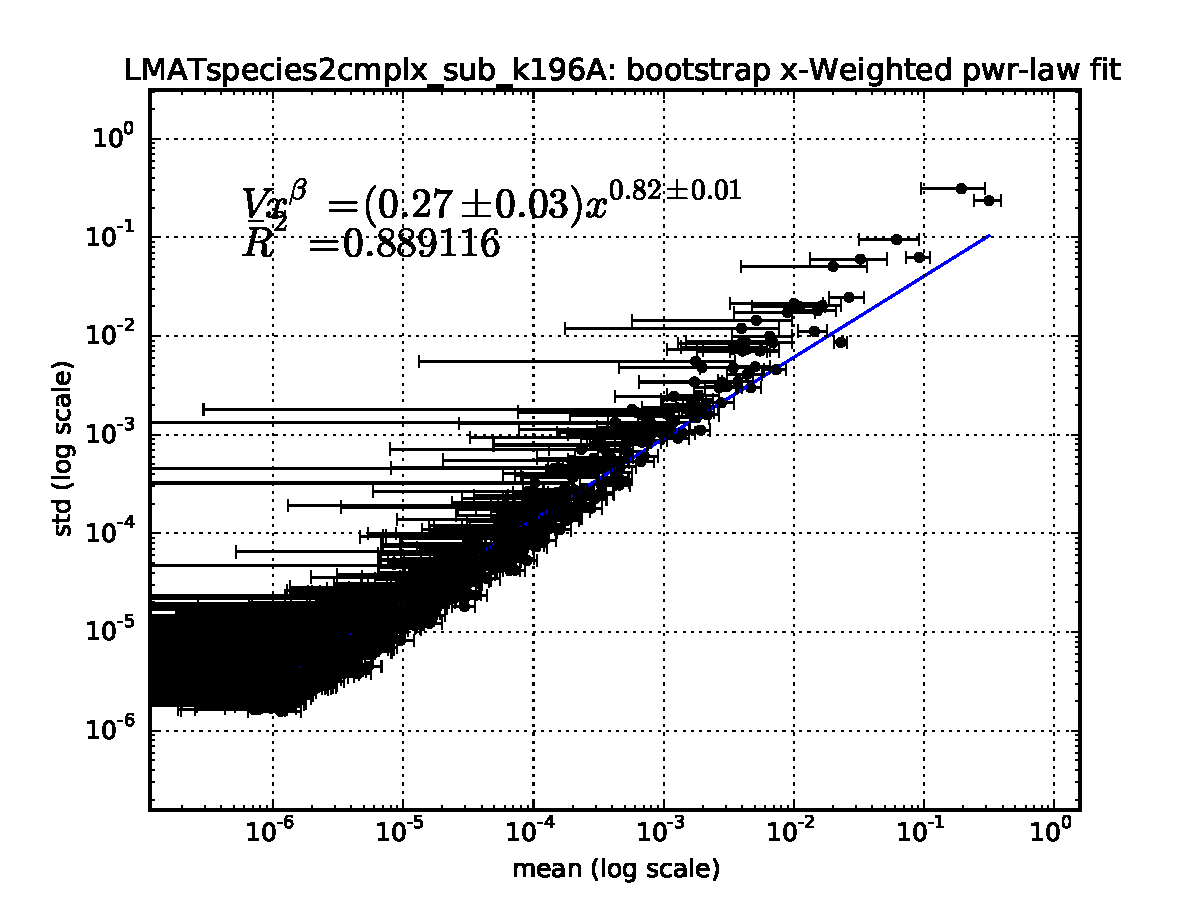
\includegraphics[width=0.5\textwidth]{results/taxalevel/xWb_spc_SMS.pdf}
\caption{Detail of comparison of different approaches based on adjacent taxonomic levels using plots of X-weighted power-law fits (see Section \ref{sec:X-w}). The former row of subfigures shows examples for 16S, whereas the latter row of subfigures plots examples for SMS. The left column shows results for the superior taxonomic level (family for 16S, genus for SMS), while the right column shows results for the inferior level (genus for 16S, specie for SMS).}
\label{fig:taxlev2}
\end{figure}



\subsection*{ComplexCruncher}

A complete software framework, named 'ComplexCruncher', has been engineered to support the analysis of the dynamics of ranking processes in complex systems. Although the software was devised with a clear bias towards metagenomics, it is general enough to be able to cope with a ranking process in any complex system. Implemented in Python using well-known open-source community software, the software solution is composed of two parts that can be used together or apart: a web-based graphic front-end connected to a database, and a computing kernel. Used together, this software enables other users to reproduce our results easily and, furthermore, upload and analyse their own data or experiment with the preloaded metagenomics data sets.

`ComplexCruncher WebPortal' (CCWebPortal) is a web platform designed to allow the user to interact with a data repository of selected and well-documented metagenomics data sources. Through a few simple steps, the user can perform advanced searches on the complete set of records in the metagenomics repository.  The web application provides advanced filters that allow the user to reduce the search to a small set of interest. After this first step, the user can refine the search and discard those records that do not meet certain requirements.

The web application allows calculations to be done directly by the stable release of the \CC\ computing kernel. At the end of the calculations, the results are displayed to the user on the same browser which runs the web application. Then, the user can interact over the series of generated graphics thus allowing flexible comparison among them. In addition, CCWebPortal enables direct download of generated data (plots, spreadsheets, etc). The web application generates a report file summarizing all the results in PDF format. If the user has login permissions, CCWebPortal enables the option of insert new database records in addition to editing and deleting existing ones.

CCWebPortal is a web application that runs on current versions of many browsers. Additional software is not needed and only requires javaScript to be enabled on the browser to run applications. 
CCWebPortal is implemented following the client$-$server distributed programming model, where the javaScript client application connects to a remote server that enables the execution of calculations and transactions through a centralized database management system. A set of relational tables allows the structuring of the metagenomics repository to establish relationships between records. Thus the search and information threshing is optimized for queries launched from the client interface. Access to the database on the server is implemented through Django framework, an open-source framework written in Python using the model-view-controller (MVC) architectural pattern for implementing user interfaces.

The effective data analysis has been performed with a Python tool developed from scratch to more than 4200 lines of code. Implemented following the Object Oriented Programming, paradigm, this software is the back-end of the website described above. However, it could be run as an independent piece of software since it is built as a Python package provided with a command-line front-end (\CC.py). Once installed, the tool can be run interactively but also in automatic mode, which uses parallel computation to speed up the analysis of several data sources. 

\CC\ performs the power-law fit described in the \emph{Blumm, N. et al.} paper, but by fitting the best model, i.e. choosing between fitting a power-law using linear regression versus nonlinear regression\cite{ecology}. In the power-law fit plots we also show the generalized coefficient of determination computed for continuous models\cite{genR2,disR2}.

\subsection*{Un-weighted power-law fit}\label{sec:unw}

\subsubsection*{Fitting the best model}

As already mentioned, to choose between fitting power laws ($y=Vx^\beta$) using linear regression on log-transformed (LLR) data versus non-linear regression (NLR), we mainly follow \emph{General Guidelines for the Analysis of Biological Power Laws}\cite{ecology}. It consists of the following three steps:
\begin{enumerate}
    \item Determining the appropriate error structure by likelihood analysis.
    \begin{enumerate}
        \item Fit the Non-Linear Regression (NLR) model and obtain $V_\text{NLR}$, $\beta_\text{NLR}$ and $\sigma_\text{NLR}^2$.
        \item Calculate the loglikelihood that the data ($n$ is sample size) are generated from a normal distribution with additive error:
        \begin{itemize}
            \item The likelihood of a normal distribution is: 
            \begin{linenomath}
            $$\mathcal{L}_\text{norm} = \prod_{i=1}^n\left[\frac{1}{\sqrt{2\pi\sigma^2_\text{NLR}}}\;\exp{\left(-\frac{\left(y_i-V_\text{NLR}x_i^{\beta_\text{NLR}}\right)^2}{2\sigma^2_\text{NLR}}\right)}\right]$$
            \end{linenomath}
            \item So, the loglikelihood of a normal distribution is:
            \begin{eqnarray*}
                \log\mathcal{L}_\text{norm} &=& -\frac{n}{2}\log\left|2\pi\sigma^2_\text{NLR}\right| - \frac{1}{2\sigma^2_\text{NLR}}\underbrace{\sum_{i=1}^n\left(y_i-V_\text{NLR}x_i^{\beta_\text{NLR}}\right)^2}_{\mathrm{RSS
                }_\text{NLR}}\\
                &=& -\frac{n}{2}\log\left|2\pi\sigma^2_\text{NLR}\right|-\frac{\mathrm{RSS}_\text{NLR}}{2\sigma^2_\text{NLR}}
            \end{eqnarray*}
        \end{itemize}
        \item Calculate the \emph{corrected Akaike's Information Criterion} for the NLR model:
		\begin{linenomath}
        $$\mathrm{AIC_{c_{NLR}}} = 2k - 2\log\mathcal{L}_\text{norm} + \frac{2k(k+1)}{n-k-1}$$
		\end{linenomath}
        \item Fit the Log-transformed Linear Regression (LLR) model and obtain $V_\text{LLR}$, $\beta_\text{LLR}$ and $\sigma_\text{LLR}^2$.
        \item Calculate the loglikelihood that the data ($n$ is sample size) are generated from a lognormal distribution with multiplicative error:
        \begin{itemize}
            \item The likelihood of a lognormal distribution is: 
            \begin{linenomath}
            $$\mathcal{L}_\text{logn} = \prod_{i=1}^n\left[\frac{1}{y_i\sqrt{2\pi\sigma^2_\text{LLR}}}\;\exp{\left(-\frac{\left(\log|y_i|-\log|V_\text{LLR}|-\beta_\text{LLR}\log|x_i|\right)^2}{2\sigma^2_\text{LLR}}\right)}\right]$$
            \end{linenomath}
            \item So, the loglikelihood of a lognormal distribution is: 
            \begin{eqnarray*}
                \log\mathcal{L}_\text{logn} &=& -\frac{n}{2}\log\left|2\pi\sigma^2_\text{LLR}\right| - \sum_{i=1}^n\log|y_i| -\\
                &&\qquad-\frac{1}{2\sigma^2_\text{LLR}}\underbrace{\sum_{i=1}^n\left(\log|y_i|-\log|V_\text{LLR}|-\beta_\text{LLR}\log|x_i|\right)^2}_{\mathrm{RSS
                }_\text{LLR}}\\
                &=& -\frac{n}{2}\log\left|2\pi\sigma^2_\text{LLR}\right| - \frac{\mathrm{RSS}_\text{LLR}}{2\sigma^2_\text{LLR}} - \sum_{i=1}^n\log|y_i|
            \end{eqnarray*}
        \end{itemize}
        \item Calculate the \emph{corrected Akaike's Information Criterion} for the LR model: 
        	\begin{linenomath}
        	$$\mathrm{AIC_{c_{LLR}}} = 2k - 2\log\mathcal{L}_\text{logn} + \frac{2k(k+1)}{n-k-1}$$
			\end{linenomath}
    \end{enumerate}
    \item Compare $\mathrm{AIC_{c_{NLR}}}$ with $\mathrm{AIC_{c_{LLR}}}$:
    \begin{itemize}
        \item If $\mathrm{AIC_{c_{NLR}}} - \mathrm{AIC_{c_{LLR}}} < -2$, the assumption of normal error is favoured compared to lognormal error, so proceed with the results obtained from the NLR fit.
        \item If $\mathrm{AIC_{c_{NLR}}} - \mathrm{AIC_{c_{LLR}}} > 2$, the assumption of lognormal error is favoured compared to normal error, so proceed with the results obtained from the LLR fit.
        \item If $\left|\mathrm{AIC_{c_{NLR}}} - \mathrm{AIC_{c_{LLR}}}\right| \leq 2$, no model is favoured, so proceed with model averaging:
        \begin{eqnarray*}
            B_\text{av} &=& w_\text{NLR}V_\text{NLR} + w_\text{LLR}V_\text{LLR} \\
            \beta_\text{av} &=& w_\text{NLR}\beta_\text{NLR} + w_\text{LLR}\beta_\text{LLR}
        \end{eqnarray*}
        where: 
        \begin{eqnarray*}
            w_\text{NLR} &=& \frac{1}{1+\mathrm{e}^{\frac{1}{2}\left(\mathrm{AIC_{c_{NLR}}}-\mathrm{AIC_{c_{LLR}}}\right)}} \\
            w_\text{LLR} &=& \frac{1}{1+\mathrm{e}^{\frac{1}{2}\left(\mathrm{AIC_{c_{LLR}}}-\mathrm{AIC_{c_{NLR}}}\right)}}
        \end{eqnarray*}
        which are obtained to fulfill the next condition: $w_\text{NLR} + w_\text{LLR} = 1$. The CIs for $B_\text{av}$ and $\beta_\text{av}$ are to be generated by ordinary bootstrapping\footnote{\CC\ has available the next bootstrapping alternatives\cite{boot}: ordinary, ``Resampling Residuals'' method, ``Wild'' method, and ``Monte-Carlo'' method.}.      
    \end{itemize}
    \item Assess the validity of the underlying statistical assumptions with diagnostic plots because while it is rare for all the assumptions to be fully satisfied by real-life data sets, major violations indicate the lack of appropriateness of the model and, thus, the potential invalidity of the results.
\end{enumerate}

\subsubsection*{Calculating the coefficient of determination}

We think the best approach in this situation is to apply the generalized $R^2$ that, for continuous models, was defined as\cite{genR2}:
\begin{linenomath}
$$ R^2 = 1 - \left(\frac{\mathcal{L}(0)}{\mathcal{L}(\hat\theta)}\right)^{\!\!\frac{2}{n}} $$
\end{linenomath}
where $\mathcal{L}(\hat\theta)$ and $\mathcal{L}(0)$  denote the likelihoods of the fitted and the ``null'' model, respectively, and $n$ is the sample size. In terms of the loglikelihoods, the generalized coefficient of determination would be:
\begin{linenomath}
$$ R^2 = 1 - \mathrm{e}^{-\frac{2}{n}\left(\log\mathcal{L}(\hat\theta)-\log\mathcal{L}(0)\right)} $$
\end{linenomath}
We have the likelihoods calculated from the previous section, but what about the ``null'' models? We understand that they are the models with only the intercept. So for the Gaussian additive error model:
\begin{linenomath}
$$\mathcal{L}_\text{norm}(0) = \prod_{i=1}^n\left[\frac{1}{\sqrt{2\pi\sigma^2_\text{NLR0}}}\;\exp{\left(-\frac{\left(y_i-\bar y\right)^2}{2\sigma^2_\text{NLR0}}\right)}\right]$$
\end{linenomath}
So:
\begin{eqnarray*}
\log\mathcal{L}_\text{norm}(0) &=& -\frac{n}{2}\log\left|2\pi\sigma^2_\text{NLR0}\right| - \frac{1}{2\sigma^2_\text{NLR0}}\sum_{i=1}^n\left(y_i-\bar y\right)^2\\
 &=& -\frac{n}{2}\left(\log\left|2\pi\sigma^2_\text{NLR0}\right| + 1 \right)
\end{eqnarray*}
since $\sigma^2_\text{NLR0}=\frac{1}{n}\sum\left(y_i-\bar y\right)^2=\frac{1}{n}\mathrm{TSS}_\text{NLR}$. Now, coming back to the coefficient of determination, we have:
\begin{eqnarray*}
R^2_\text{NLR} &=& 1 - \mathrm{e}^{\frac{2}{n}\left(\log\mathcal{L}_\text{NLR}(0)-\log\mathcal{L}_\text{NLR}(\hat\theta)\right)} = 1 - \exp{\left(\frac{\log(\mathrm{RSS}_\text{NLR})}{\log(\mathrm{TSS}_\text{NLR})}\right)}
 =\\ &=& 1 - \frac{\mathrm{RSS}_\text{NLR}}{\mathrm{TSS}_\text{NLR}} =
 1 - \frac{\sum_{i=1}^n\left(y_i-V_\text{NLR}x_i^{\beta_\text{NLR}}\right)^2}{\sum_{i=1}^n\left(y_i-\bar y\right)^2}
\end{eqnarray*}
recovering the traditional expression for $R^2$. Using the same approach for calculating $R^2_\text{LLR}$, then:
\begin{linenomath}
$$\mathcal{L}_\text{logn}(0) = \prod_{i=1}^n\left[\frac{1}{y_i\sqrt{2\pi\sigma^2_\text{LLR0}}}\;\exp{\left(-\frac{\left(\log|y_i|-\log|B_\text{LLR0}|\right)^2}{2\sigma^2_\text{LLR0}}\right)}\right]$$
\end{linenomath}
So:
\begin{eqnarray*}
\log\mathcal{L}_\text{logn}(0) &=& -\frac{n}{2}\log\left|2\pi\sigma^2_\text{LLR0}\right| - \frac{1}{2\sigma^2_\text{LLR0}}\sum_{i=1}^n\left(\log|y_i|-\overline{\log|y|}\right)^2 - \sum_{i=1}^n\log|y_i|\\
 &=& -\frac{n}{2}\left(\log\left|2\pi\sigma^2_\text{LLR0}\right| + 1 \right) - \sum_{i=1}^n\log|y_i|
\end{eqnarray*}
since $\sigma^2_\text{LLR0}=\frac{1}{n}\sum\left(\log|y_i|-\overline{\log|y|}\right)^2=\frac{1}{n}\mathrm{TSS}_\text{logn}$. Again, recalling the expression for the generalized coefficient of determination, we have:
\begin{eqnarray*}
R^2_\text{LLR} &=& 1 - \mathrm{e}^{\frac{2}{n}\left(\log\mathcal{L}_\text{LLR}(0)-\log\mathcal{L}_\text{LLR}(\hat\theta)\right)} = 1 - \exp{\left(\frac{\log(\mathrm{RSS}_\text{LLR})}{\log(\mathrm{TSS}_\text{LLR})}\right)}
 =\\ &=& 1 - \frac{\mathrm{RSS}_\text{LLR}}{\mathrm{TSS}_\text{LLR}} =
 1 - \frac{\sum_{i=1}^n\left(\log|y_i|-\log|V_\text{LLR}|-\beta_\text{LLR}\log|x_i|\right)^2}{\sum_{i=1}^n\left(\log|y_i|-\overline{\log|y|}\right)^2}
\end{eqnarray*}


\subsection*{X-weighted power-law fit}\label{sec:X-w}

When fitting the power-law of std vs. mean, we can take into account that every mean has uncertainty and estimate it for a sample size $n$ by the SEM (\emph{Standard Error of the Mean}):
\begin{linenomath}
$$ \mathrm{SEM} = \frac{s}{\sqrt{n}}$$
\end{linenomath}
where $s$ is the sample standard deviation. So, the vector of weights is computed with:
\begin{linenomath}
$$ \mathbf{w} = \frac{1}{\overrightarrow{\mathrm{SEM}}} = \frac{\sqrt{\mathbf{n}}}{\mathbf{s}}$$
\end{linenomath}

Here, the uncertainties affect the independent variable, so the fit is not so trivial as a Y-weighted fit, where the uncertainties affect the dependent variable. A standard approach to do this fit is: a) invert your variables before applying the weights, b) then perform the weighted fit, and finally, c) revert the inversion. This method is deterministic, but the approximate solution worsens with smaller $R^2$. For comparison, we develop a stochastic method by using a bootstrapping-like strategy that avoids the inversion and is applicable regardless of $R^2$. Both methods, detailed below, are implemented in \CC.

\subsubsection*{Method 1: By inverting the data}

In the case of the log-LR model, we have:
\begin{linenomath}
$$\log y = \log V + \beta\log x \quad\rightarrow\quad \underbrace{\log x}_{\tilde y} = \overbrace{-\frac{1}{\beta}\log V}^{b} + \overbrace{\frac{1}{\beta}}^{m}\underbrace{\log y}_{\tilde x}$$ 
\end{linenomath}
where $m$ determines the slope or gradient of the fitted line, and $b$ determines the point at which the line crosses the y-axis, otherwise known as the y-intercept. Once the model is fitted, the original parameters can be retrieved easily:
\begin{eqnarray*}
\beta &=& \frac{1}{m} \\
V &=& \mathrm{e}^{-\beta b} = \mathrm{e}^{-\frac{b}{m}}
\end{eqnarray*}
Their respective uncertainties are to be obtained using \emph{error propagation}:
\begin{eqnarray*}
    \sigma_\beta &=& \left|\frac{\mathrm{d}\beta}{\mathrm{d}m}\right|\sigma_m \quad=\quad \frac{1}{m^2}\;\sigma_m \\
    \sigma_V &=& \sqrt{\left(\frac{\partial V}{\partial b}\right)^{\!\!2}\sigma_b^2 +
      \left(\frac{\partial V}{\partial m}\right)^{\!\!2}\sigma_m^2} \quad=\quad
      \frac{1}{m}\;\mathrm{e}^{-\frac{b}{m}}\,\sqrt{\sigma_b^2 + \frac{b^2}{m^2}\;\sigma_m^2} 
\end{eqnarray*}

\subsubsection*{Method 2: Bootstrapping-like strategy}

The basic idea of bootstrapping is that inference about a population from sample data (sample $\rightarrow$ population) can be modeled by resampling the sample data and performing inference on (resample $\rightarrow$ sample). To adapt this general idea to our problem, we resample the x-data array using its errors array. That is, for each replicate, a new x-data array is computed based on:
\begin{linenomath}
$$x^*_i = x_i + v_i$$
\end{linenomath}
where $v_i$ is a Gaussian random variable with mean $\mu_i=0$ and standard deviation $\sigma_i=\mathrm{SEM}_i$, as defined previously in this supplementary material. For each replicate a complete un-weighted power-law fit is performed, as described in the previous section. It is worth mentioning that each replicate is filtered to avoid values of $x^*_i$ under \emph{eps} (obtained by \texttt{np.finfo(np.double).eps}) in order to keep away from the error of getting log of negatives or zero during the fit.

We devised and implemented a multi-step algorithm to estimate the fit parameters that finishes when a relative error of less than $10^{-4}$ is achieved. It also ends if the number of steps reaches $100$ to avoid too much time lapse, to prevent any pathologic numeric case which, in fact, we still have not detected in all the data sets analyzed.

In the previous version of the algorithm, for each step, the method generated $10$ replicates for each x-data point, in other words, it was computing the fit for $10$ times the length of the x-data array replicates, with a maximum of $10000$ fits per step. Nevertheless, we found that such an approach depending on the length of the x-data array did not perform better, so we decided to simplify the method and fix the number of fits per step in $100$. This latter approach improved the performance. 

The parameters of the X-weighted fit are then estimated by averaging through all the replicate fits performed, and their errors are estimated by computing the standard deviation also for all the fits. At the end of each step, the relative error is calculated by comparing the fit parameters estimation in the last step with the previous one.

Finally, both the coefficient of determination of the fit and the coefficient of correlation between the fit parameters are estimated by averaging.

\subsection*{Rank Stability Index (RSI)}\label{sec:RSI}

The Rank Stability Index is shown as a percentage in a separate bar on the right of the rank matrix plot provided by \CC. The RSI is strictly $1$ for an element whose range never changes over time, and is strictly $0$ for an element whose rank oscillates between the extremes from time to time. So, RSI is calculated, per element, as $1$ less the quotient of the number of true rank hops taken between the number of maximum possible rank hops, all powered to $p$:
\begin{linenomath}
$${\rm RSI} = \left(1-\frac{\text{true rank hops}}{\text{possible rank hops}}\right)^p = \left(1-\frac{D}{(N-1)(t-1)}\right)^p$$
\end{linenomath}
where $D$ is the total of rank hops taken by the studied element, $N$ is the number of elements that have been ranked, and $t$ is the number of time samples. The power index $p$ is arbitrarily chosen to increase the resolution in the stable region; the value in the current version of the code is $p=4$. 

As an example of this ``zooming'' effect in the stable region, to match a linear ($p=1$) RSI of 0.9 to a powered one of 0.1, we should select $p=21.8543$. An alternative way to obtain this effect and exactly map a linear RSI of 0.9 to a non-linear RSI (${\rm RSI'}$) of 0.1, is by applying the following function:
\begin{linenomath}
$${\rm RSI'} = \frac{10^{10\left(1-\frac{D}{(N-1)(t-1)}\right)}-1}{10^{10}-1} \approx 10^{-10\left(\frac{D}{(N-1)(t-1)}\right)}$$
\end{linenomath}
where the approximation is valid because $10^{10}\gg 1$ but, the small price to pay for it is that, in the worst instability case, the ${\rm RSI'}$ would not be strictly $0$ but $10^{-10}$.

The colour code of the RSI percentage text in the rank plot of \CC\ is chosen following the first condition satisfied from those shown in Table \ref{tab:RSI} (see page \pageref{tab:RSI}). 

\begin{table}
  \begin{center}
    \begin{tabular}{ccc}
    \hline
    Case  &  Condition  &  Colour  \\
    \hline
    1  &  $1\ge{\rm RSI}>0.99$  & \textcolor{blue}{blue}  \\ 
    2  & ${\rm RSI}>0.90$  &  \textcolor{green}{green}  \\
    3  &  ${\rm RSI}>0.75$  &  \textcolor{orange}{orange} \\
    4  &  ${\rm RSI}>0.25$  &  \textcolor{red}{red} \\
    5  &  $0.25\ge{\rm RSI}\ge0$  &  \bfseries{black}  \\
    \hline
    \end{tabular}
  \end{center}
  \caption{Colour code of the RSI percentage text shown in rank plots, following the first condition satisfied.}
  \label{tab:RSI}
\end{table}

\subsection*{\CC\ output}
In the previous sections, we have discussed details about the methods used in \CC. In this section we review the output from the package, which aims at summarizing the as yet undescribed functionality. 

\subsubsection*{Fit Plots}
Both for the unweighted fit (detailed in the section \ref{sec:unw}) and for the X-weighted fit (detailed in the section \ref{sec:X-w}), two plots are generated: the former with logarithmic scale, the latter with lineal scale. Figure \ref{fig:unwFit} shows an example of the unweighted fit plots and Figure \ref{fig:X-wFit} does the same with the X-weighted fit plots. Additionally, for the unweighted fit, a complete residues analysis is performed, and a 4-in-1 figure is generated as shown in Figure \ref{fig:unwRes}, corresponding to the fit of Figure \ref{fig:unwFit}. Among other tests, it allows to check for normality and homoscedasticity of the residues.

\begin{figure}
	\centering
	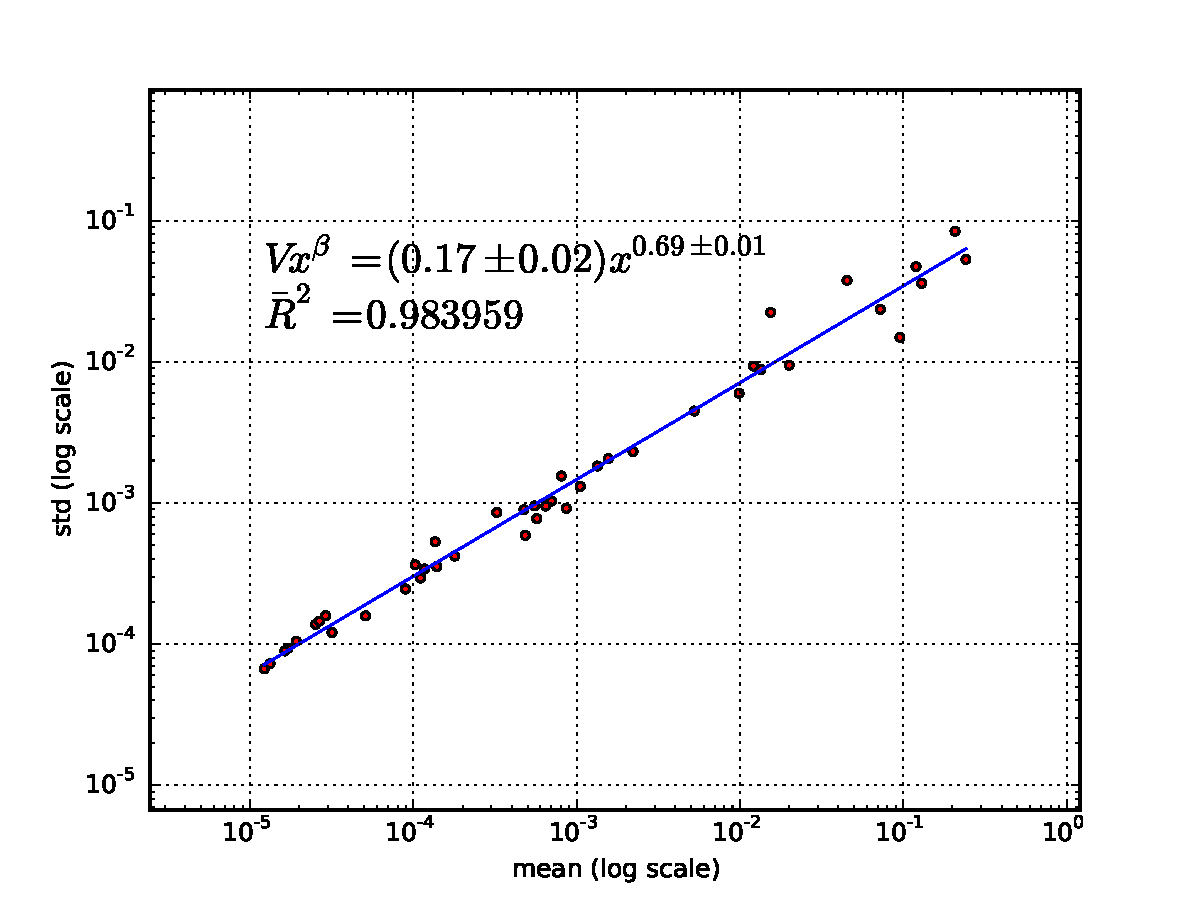
\includegraphics[width=0.8\textwidth]{results/fits/IBS_h_A_amplicons_family_stdVSmean_LLR_LOG.pdf}
	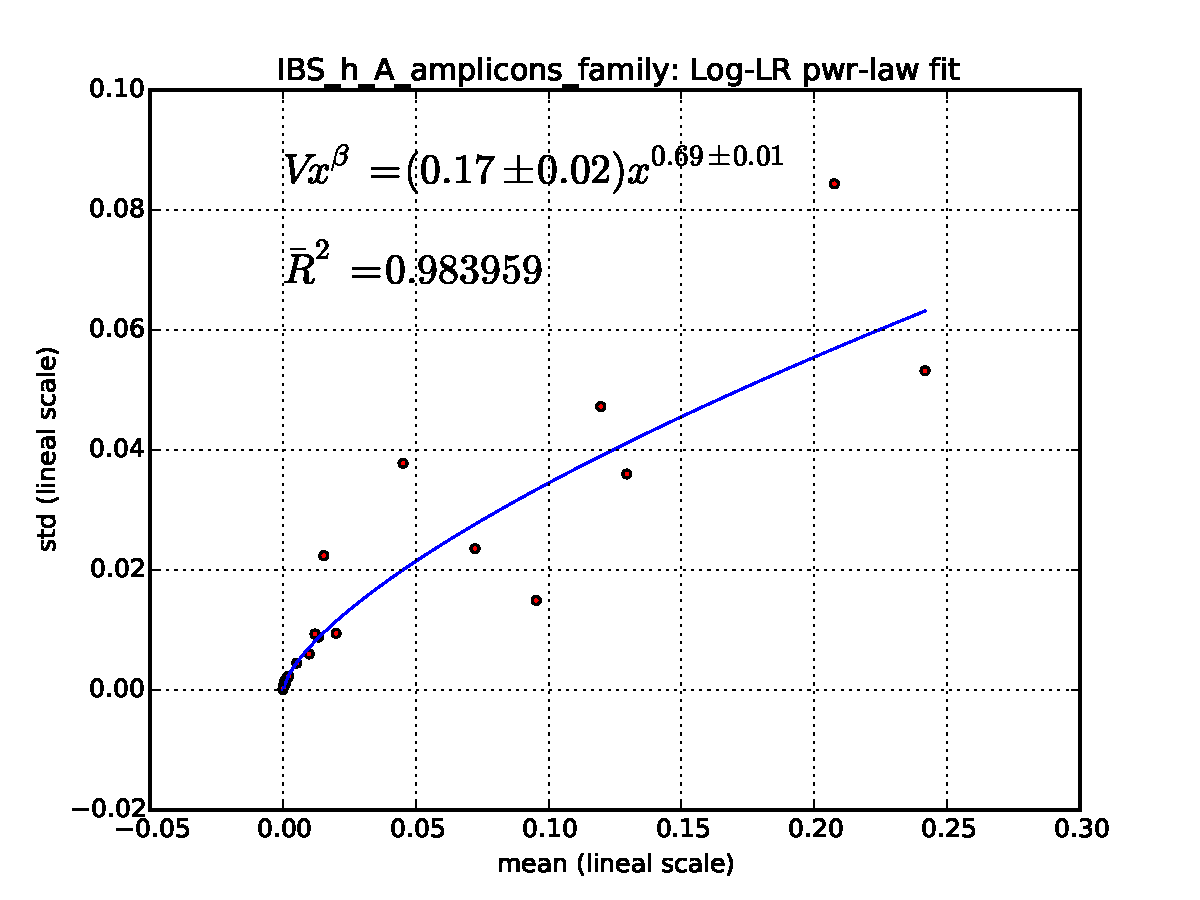
\includegraphics[width=0.8\textwidth]{results/fits/IBS_h_A_amplicons_family_stdVSmean_LLR_LIN.pdf}
	\caption{Example of unweighted fit, shown both in logarithmic and lineal scale plots}
	\label{fig:unwFit}
\end{figure}

\begin{figure}
	\centering
	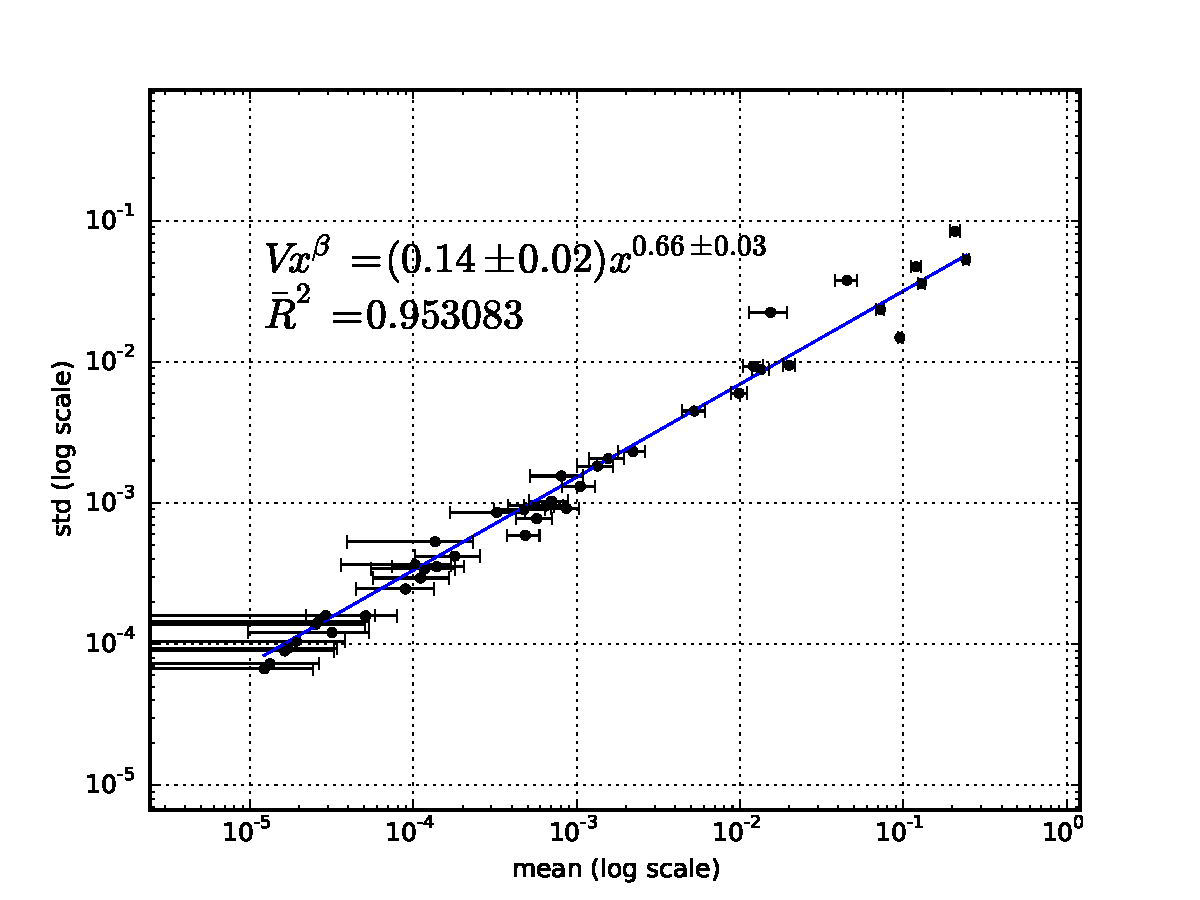
\includegraphics[width=0.8\textwidth]{results/fits/IBS_h_A_amplicons_family_stdVSmean_xWboot_LOG.pdf}
	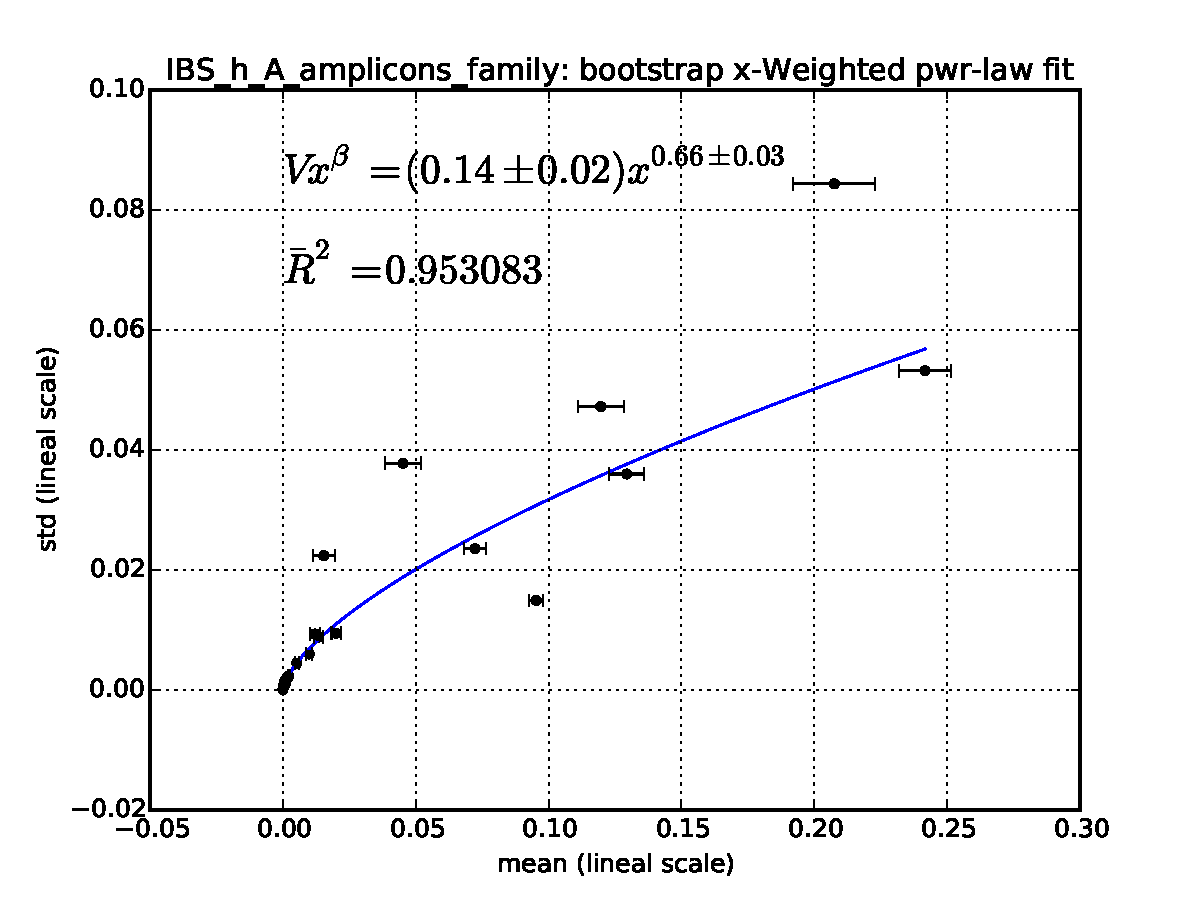
\includegraphics[width=0.8\textwidth]{results/fits/IBS_h_A_amplicons_family_stdVSmean_xWboot_LIN.pdf}
	\caption{The X-weighted fit log and lineal plots corresponding to the fit of Figure \ref{fig:unwFit}}
	\label{fig:X-wFit}
\end{figure}

\begin{figure}
	\centering
	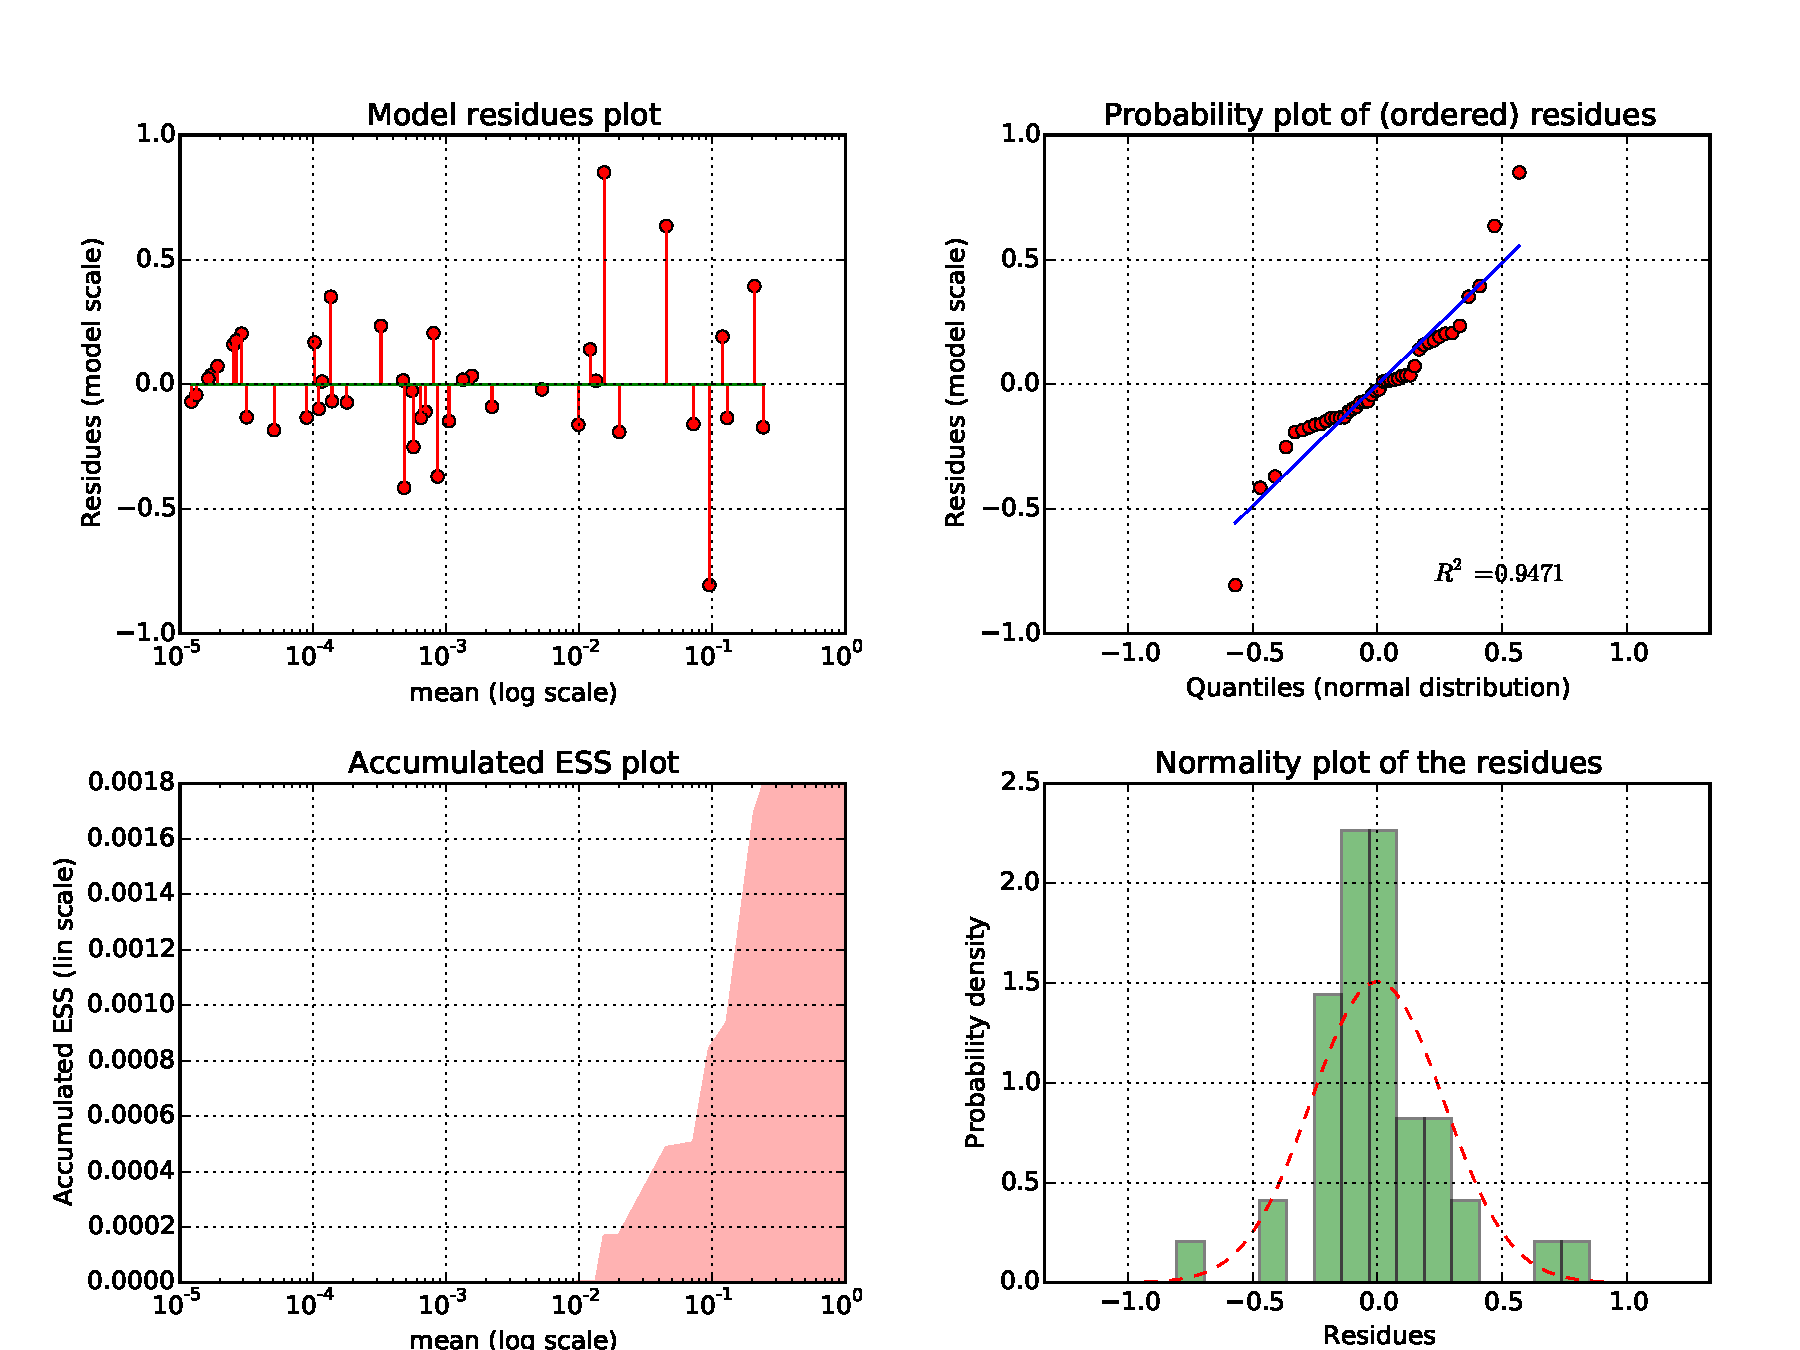
\includegraphics[width=\textwidth]{results/fits/IBS_h_A_amplicons_family_stdVSmean_LLR_RES.pdf}
	\caption{Residues analysis plot corresponding to the fit of Figure \ref{fig:unwFit}. The top-left subplot is a simple residues plot. The top-right subplot is a Normal quantiles plot with linear fitting (value of coefficient of determination is provided). The bottom-left subplot shows an accumulated ESS (Explained Sum of Squares) plot. Finally, the bottom-right subplot is a residues Normal histogram plot. This set of subplots allows to check for normality and homoscedasticity of the residues.}
	\label{fig:unwRes}
\end{figure}

\subsubsection*{Histogram Plots} 
\CC\ generates three different histogram plots:
\begin{description}
	\item[$-$Absolute frequencies plot]: This plot is useful to visually assess the validity of the time points in terms of the accumulated absolute frequency of the elements (taxa), since absolute frequencies far (much higher or much lower) from those typically observed could mean a sampling problem. As an example, Figure \ref{fig:histAFP} shows this histogram for the pre-treatment data (first 7 times) of patient ``D'' in the antibiotics study\cite{antibiotic}. 
	\item[$-$2D deviation plot]: The 2D semi-logarithmic histogram representing deviations from the mean versus the mean itself, is a useful tool in the analysis of the stability of ranking processes in complex systems\cite{ranking}. Figure \ref{fig:hist2D} shows this plot for the data used in the fit shown in Figure \ref{fig:unwFit}.
	\item[$-$Zero relative frequency plot]: We could define the ZRF (Zero Relative Frequency, thereby ranging from 0 to 1) of an element (taxon) as the portion of times where it is zero, i.e., it is not found. Attending to all the elements (taxa), we can plot the ZRF histogram, which then lies on the horizontal axis of the plot. The vertical axis shows the number of elements (taxa), so the height of a bar represents the number of elements that have determinate ZRF. In this respect, the bar over $0.0$ counts the number of elements (taxa) that are present at every time point of the data set (aka ``core''), while the bar over $1.0$ would count the number of elements (taxa) that are never found (this bar never appears because all these ``null'' elements are automatically filtered by the code). Figure \ref{fig:histZRF} shows an example of this plot. There, we can see that $12$ taxa are present at all the time points of the time series while $9$ taxa basically appear only once. So, this plot is clearly useful to notice how the ``core'' is distributed.
\end{description}

\begin{figure}
	\centering
	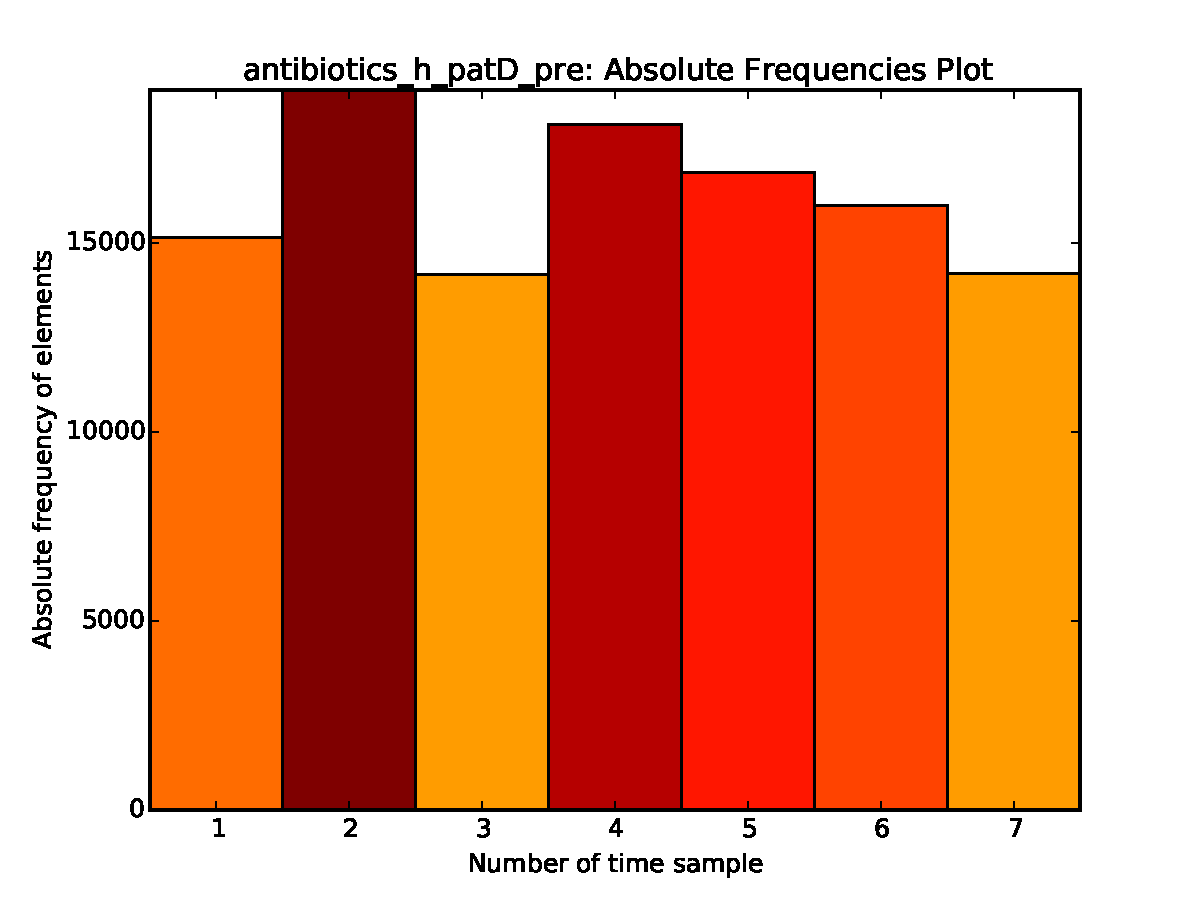
\includegraphics[width=0.8\textwidth]{results/hist/antibiotics_h_patD_pre_AbsFreqPlot}
	\caption{Histogram with the absolute frequencies of the pre-treatment data (7 first times) of patient ``D'' in the antibiotics study\cite{antibiotic}}
	\label{fig:histAFP}
\end{figure}

\begin{figure}
	\centering
	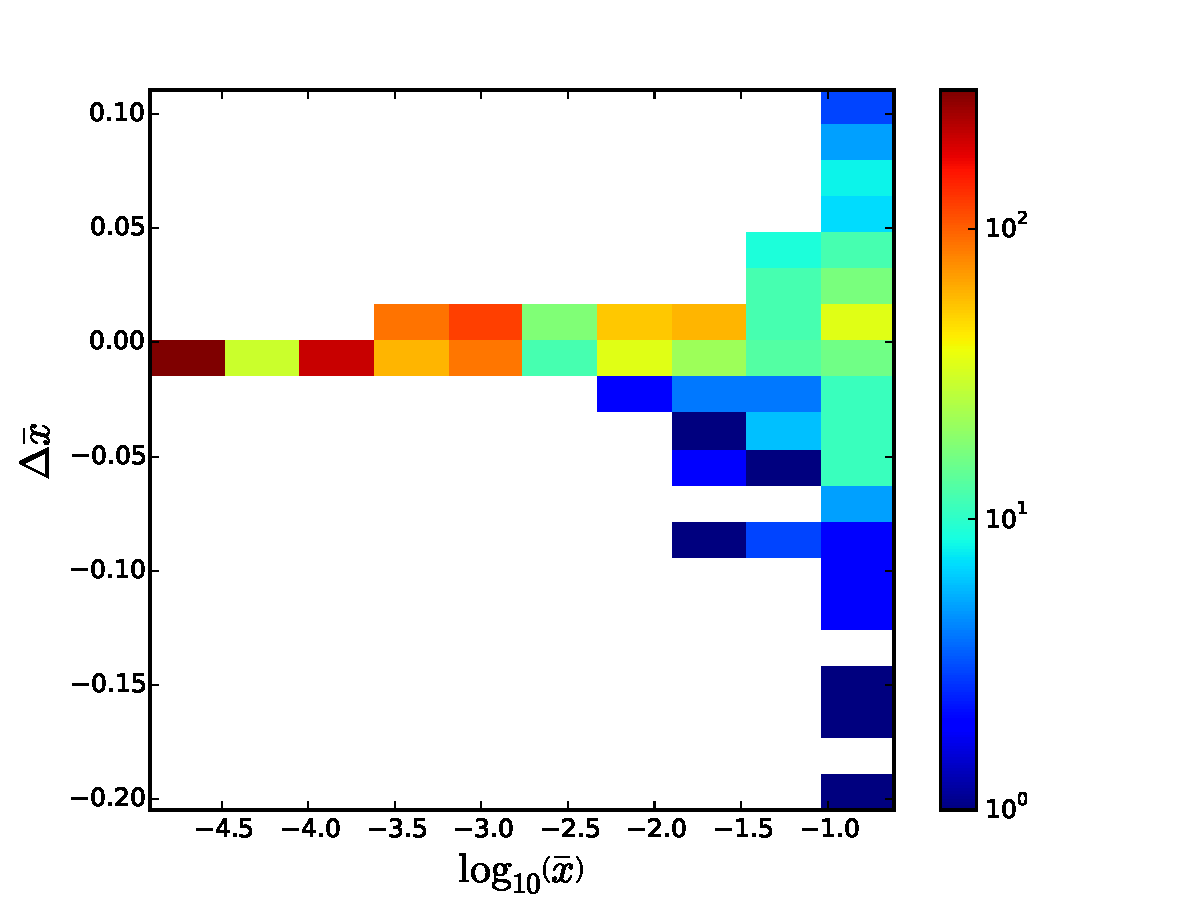
\includegraphics[width=0.8\textwidth]{results/hist/IBS_h_A_amplicons_family_hist2D.pdf}
	\caption{2D histogram deviation plot of the data used in the fit shown in Figure \ref{fig:unwFit}}
	\label{fig:hist2D}
\end{figure}

\begin{figure}
	\centering
	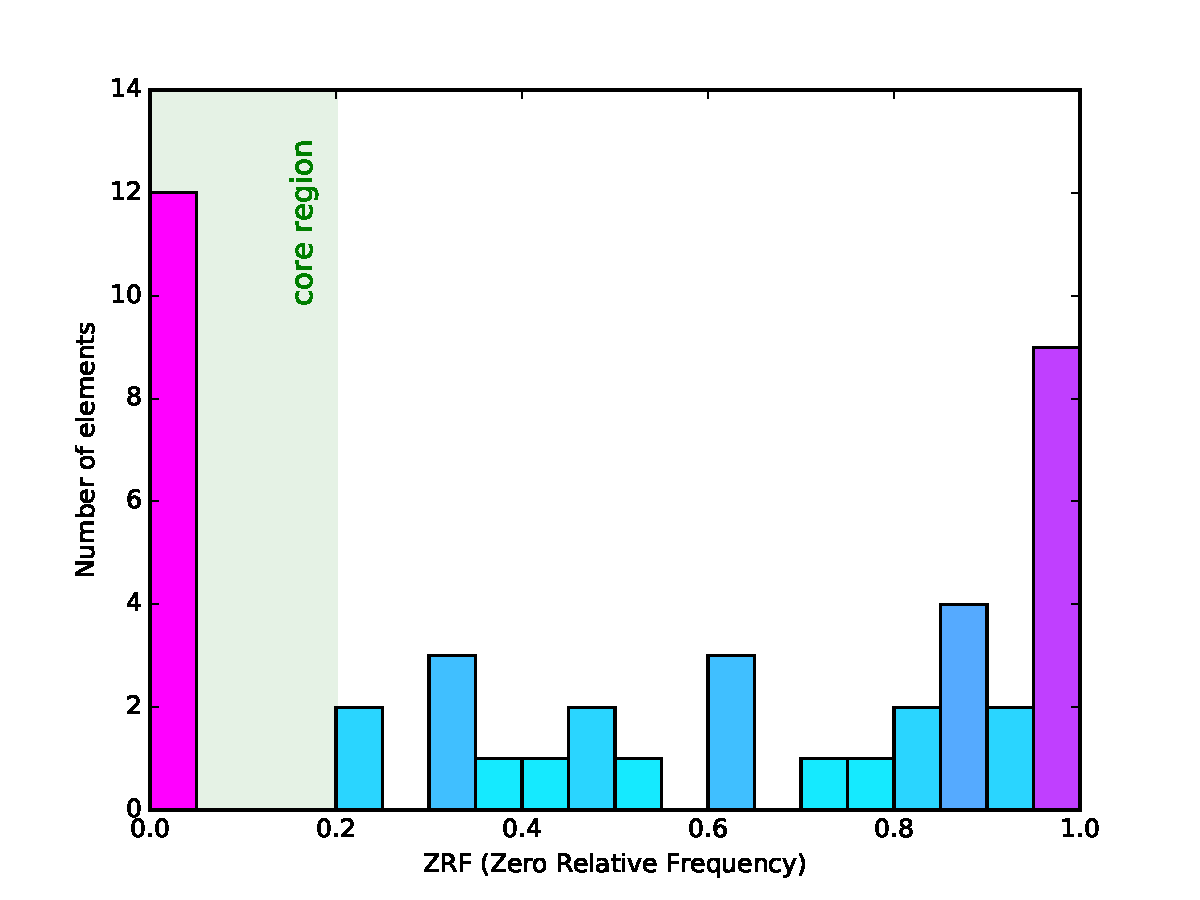
\includegraphics[width=0.8\textwidth]{results/hist/IBS_h_A_amplicons_family_ZRFhist.pdf}
	\caption{Histogram with the relative frequency of zero for the elements (taxa) in the data used in the fit shown in Figure \ref{fig:unwFit}}
	\label{fig:histZRF}
\end{figure}

\subsubsection*{Correlation and Rank Plots} 
\CC\ generates three different plots falling under this category, as well as Excel files with the resulting matrices:
\begin{description}
	\item[$-$Elements correlation matrix]: This plot shows a correlation matrix among the elements (taxa), calculated with the time as independent variable. For these calculations, the data set is not normalized to avoid entering an additional constraint. As an example, Figure \ref{fig:corrElm} shows this matrix for the ``core'' elements (taxa) present in the pre-treatment data (first seven times) of patient ``D'' in the antibiotics study\cite{antibiotic}. 
	\item[$-$Times correlation matrix]: This plot presents a correlation matrix among the time points of the data set, calculated with the elements (taxa) as independent variable. Again, the data set is not normalized. Figure \ref{fig:corrTim} shows this matrix for the ``core'' elements (taxa) present in pre-treatment data (first seven times) of patient ``D'' in the antibiotics study\cite{antibiotic}. 
	\item[$-$Rank dynamics and stability plot]: This plot shows the variation in the rank with time for the most dominant elements (taxa) and their calculated RSI, as discussed in Section \ref{sec:RSI}. Figure \ref{fig:corrank} shows this plot for the elements (taxa) in the data used in the fit shown in Figure \ref{fig:unwFit}.
\end{description}

\begin{figure}
	\centering
	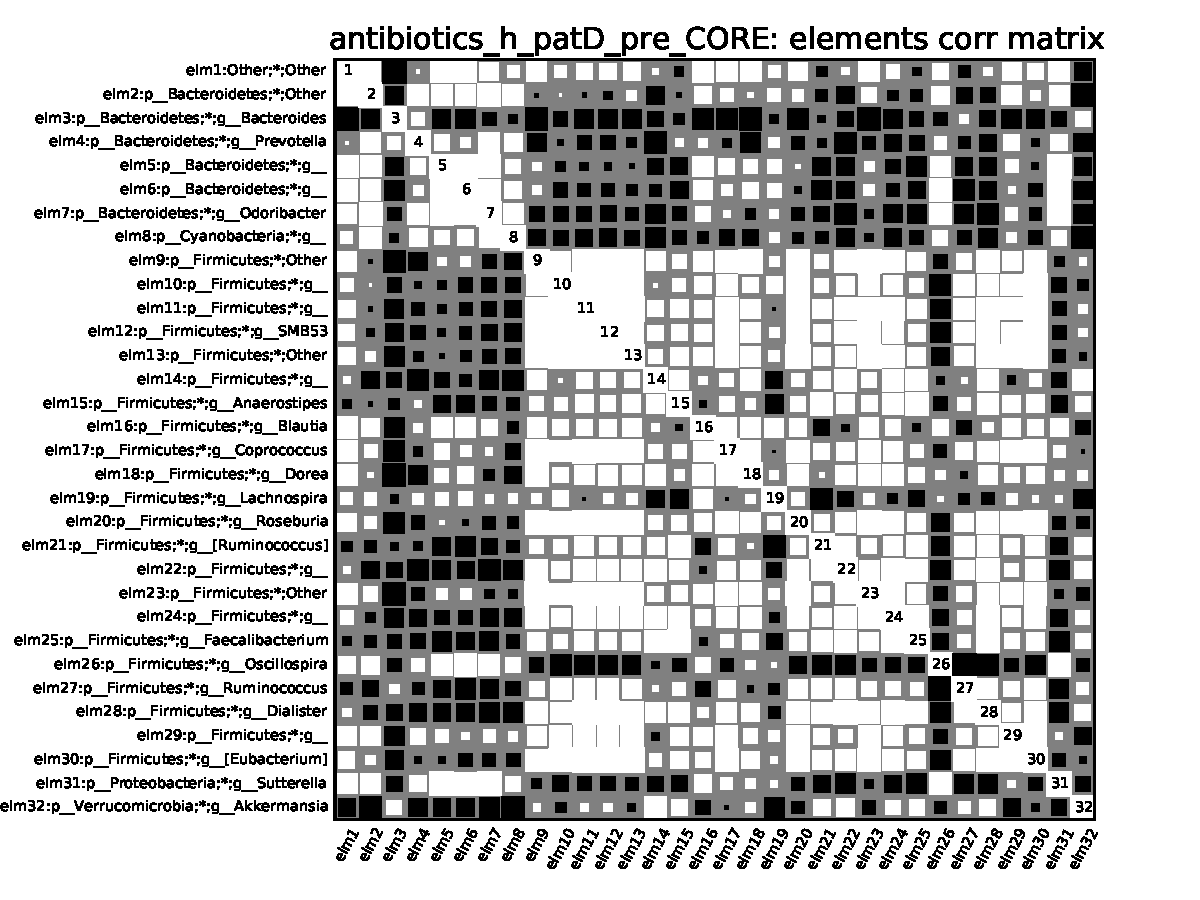
\includegraphics[width=0.9\textwidth]{results/corrank/antibiotics_h_patD_pre_CORE_ElementsCorr}
	\caption{Element correlation plot of the pre-treatment data (first seven times) of patient ``D'' in the antibiotics study\cite{antibiotic} for ``core'' taxa}
	\label{fig:corrElm}
\end{figure}

\begin{figure}
	\centering
	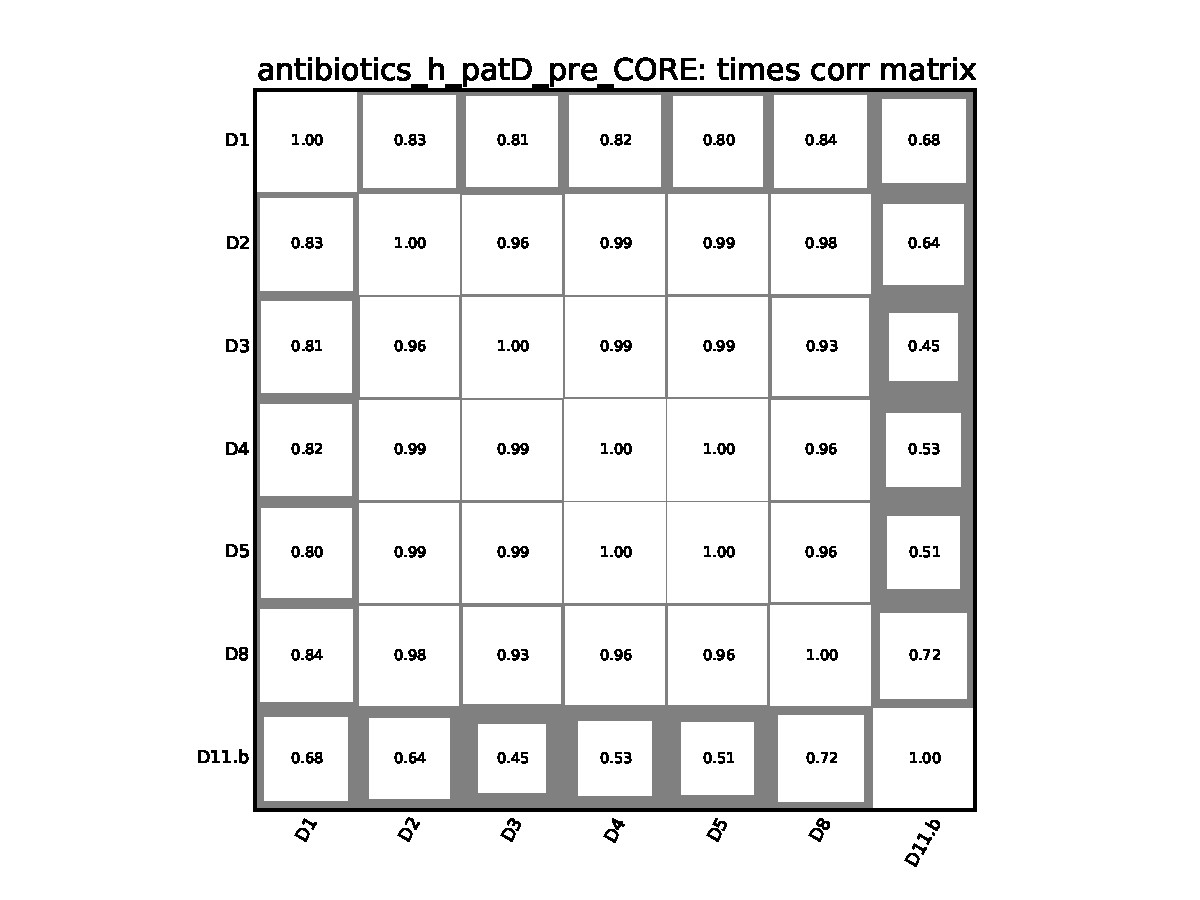
\includegraphics[width=0.9\textwidth]{results/corrank/antibiotics_h_patD_pre_CORE_TimesCorr}
	\caption{Times correlation plot of the pre-treatment data (first seven times) of patient ``D'' in the antibiotics study\cite{antibiotic} for ``core'' taxa}
	\label{fig:corrTim}
\end{figure}

\begin{figure}
	\centering
	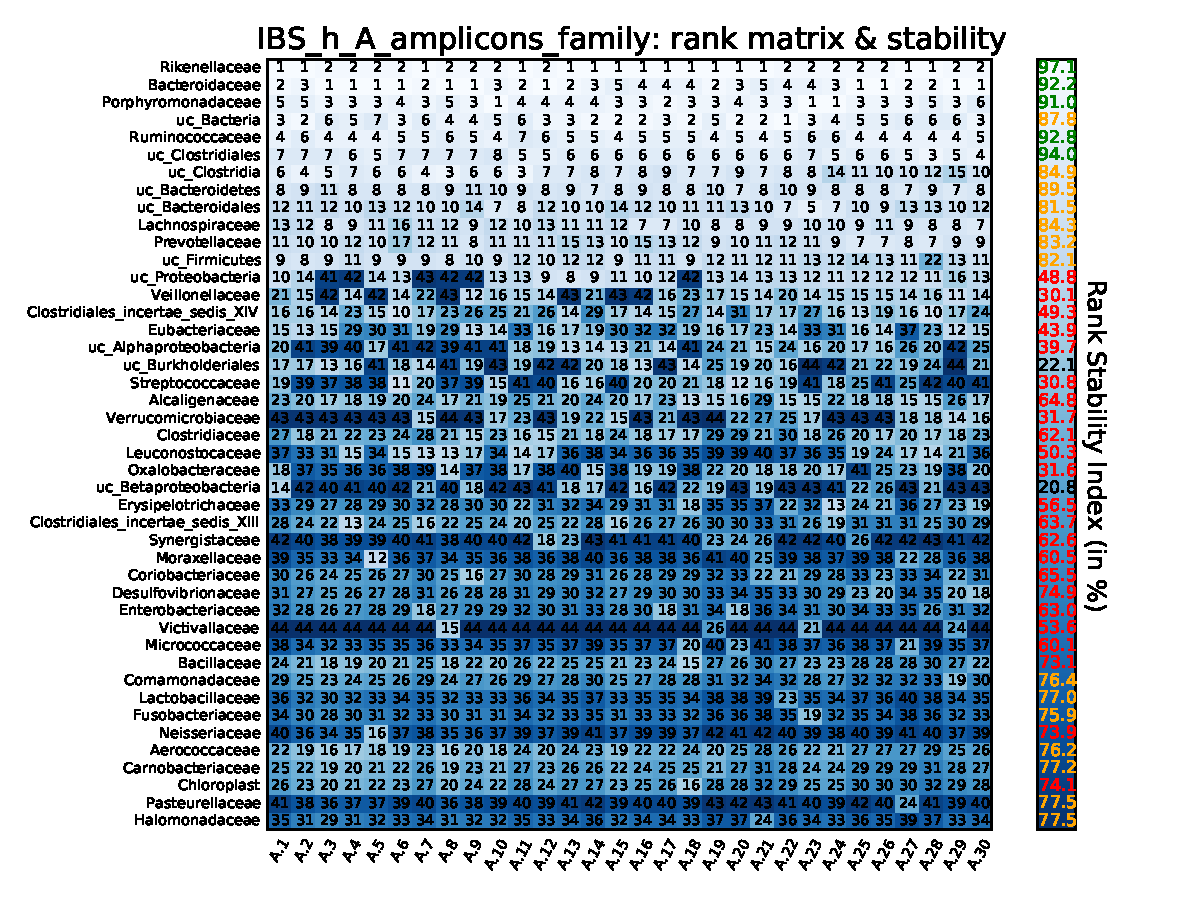
\includegraphics[width=\textwidth]{results/corrank/IBS_h_A_amplicons_family_Rank}
	\caption{Matrix showing the rank variation throughout time for the most dominant elements (taxa) and their calculated RSI (as discussed in Section \ref{sec:RSI}) in the data used in the fit shown in Figure \ref{fig:unwFit}}
	\label{fig:corrank}
\end{figure}

\subsection*{Standardization} \label{sec:stan}
In order to show all the studies properly under common axes, we decided to standardize the Taylor parameters using the group of healthy individuals for each study. With this approach, all the studies can be visualized in a shared plot with units of Taylor-parameters standard-deviation on their axes.

For a Taylor parameter, e.g. $V$, the estimate of the mean ($\widehat{V}$) for the healthy subpopulation, composed of $h$ individuals, is:
\begin{linenomath}
$$\widehat{V} = \frac{1}{W_1}\sum_{i=1}^h V_i \omega_i=\sum_{i=1}^h V_i \omega_i$$
\end{linenomath}
as $W_1=\sum_i^h \omega_i=1$, since $\omega_i$ are normalized weights calculated as:
\begin{linenomath}
$$\omega_i = \frac{\frac{1}{\sigma^2_{V_i}}}{\sum_i^h\frac{1}{\sigma^2_{V_i}}}$$
\end{linenomath}
being $\sigma_{V_i}$ the estimation of the uncertainty in $V_i$ obtained together with $V_i$ from the X-weighted power-law fit described in Section \ref{sec:X-w}, for healthy individuals.

Likewise, the estimation of the standard deviation for the healthy population ($\widehat{\sigma}_V$) is:
\begin{linenomath}
$$\widehat{\sigma}_V = \sqrt{\frac{1}{W_1-\frac{W_2}{W_1}}\sum_{i=1}^h\left[\omega_i\left(V_i-\hat{V}\right)^2\right]}$$
\end{linenomath}
being $W_2=\sum_i^h \omega_i^2$, which finally yields to:
\begin{linenomath}
$$\widehat{\sigma}_V = \sqrt{\frac{1}{1-\sum_i^h \omega_i^2}\sum_{i=1}^h\left[\omega_i\left(V_i-\hat{V}\right)^2\right]}$$
\end{linenomath}
   
\clearpage

\section*{Acknowledgments}
Authors declare that there are no competing financial interests in relation to the work described here. We thereby express our acknowledgement to Bull/Atos and Micron Technology for providing us with the PCIe SSD card Micron P420m HHHL as a free-of-charge sample for high performance throughput database testing purposes.

\section*{Funding Information}
This work is supported by Generalitat Valenciana Prometeo Grants II/2014/050, II/2014/065, by the Spanish Grants FPA2011-29678, BFU2012-39816-C02-01 of MINECO and by PITN-GA-2011-289442-INVISIBLES. JMM \& DMM acknowledge FPI and FISABIO fellowships. \todo{Modificar becas de JMM y DMM ¿poner algún grant más?}

\clearpage
\begin{thebibliography}{99}
\bibitem{holo1} {\bf Rosenberg E, Zilber-Rosenberg I.} 2016. Microbes Drive Evolution of Animals and Plants: the Hologenome Concept. MBio {\bf 7}:e01395–15–.
\bibitem{holo2} {\bf Bordenstein SR, Theis KR.} 2015. Host Biology in Light of the Microbiome: Ten Principles of Holobionts and Hologenomes. PLOS Biol {\bf 13}:e1002226.
\bibitem{holo3} {\bf Moran NA, Sloan DB.} 2015. The Hologenome Concept: Helpful or Hollow? PLoS Biol {\bf 13}:1–10.
\bibitem{bileacids} {\bf Swann JR, Want EJ, Geier FM, Spagou K, Wilson ID, Sidaway JE, Nicholson JK, Holmes E.} 2011. Systemic gut microbial modulation of bile acid metabolism in host tissue compartments. Proc Natl Acad Sci {\bf 108}:4523–4530.
\bibitem{choline} {\bf Spencer MD, Hamp TJ, Reid RW, Fischer LM, Zeisel SH, Fodor AA.} 2011. Association between composition of the human gastrointestinal microbiome and development of fatty liver with choline deficiency. Gastroenterology {\bf 140}:976–986.
\bibitem{scfa1} {\bf Samuel BS, Shaito A, Motoike T, Rey FE, Backhed F, Manchester JK, Hammer RE, Williams SC, Crowley J, Yanagisawa M, Gordon JI}. 2008. Effects of the gut microbiota on host adiposity are modulated by the short-chain fatty-acid binding G protein-coupled receptor, Gpr41. Proc Natl Acad Sci {\bf 105}:16767–16772.
\bibitem{scfa2} {\bf Smith PM, Howitt MR, Panikov N, Michaud M, Gallini CA, Bohlooly-Y M, Glickman JN, Garrett WS.} 2013. The Microbial Metabolites, Short-Chain Fatty Acids, Regulate Colonic Treg Cell Homeostasis. Science (80- ) {\bf 341}:569–573.
\bibitem {scfa3} {\bf Kimura I, Ozawa K, Inoue D, Imamura T, Kimura K, Maeda T, Terasawa K, Kashihara D, Hirano K, Tani T, Takahashi T, Miyauchi S, Shioi G, Inoue H, Tsujimoto G.} 2013. The gut microbiota suppresses insulin-mediated fat accumulation via the short-chain fatty acid receptor GPR43. Nat Commun {\bf 4}:1829.
\bibitem {scfa4} {\bf Maslowski KM, Vieira AT, Ng A, Kranich J, Sierro F, Di Yu, Schilter HC, Rolph MS, Mackay F, Artis D, Xavier RJ, Teixeira MM, Mackay CR.} 2009. Regulation of inflammatory responses by gut microbiota and chemoattractant receptor GPR43. Nature {\bf 461}:1282–1286.
\bibitem{diabetes2} {\bf Qin J, Li Y, Cai Z, Li S, Zhu J, Zhang F, Liang S, Zhang W, Guan Y, Shen D, Peng Y, Zhang D, Jie Z, Wu W, Qin Y, Xue W, Li J, Han L, Lu D, Wu P, Dai Y, Sun X, Li Z, Tang A, Zhong S, Li X, Chen W, Xu R, Wang M, Feng Q, Gong M, Yu J, Zhang Y, Zhang M, Hansen T, Sanchez G, Raes J, Falony G, Okuda S, Almeida M, LeChatelier E, Renault P, Pons N, Batto J-M, Zhang Z, Chen H, Yang R, Zheng W, Li S, Yang H, Wang J, Ehrlich SD, Nielsen R, Pedersen O, Kristiansen K, Wang J.} 2012. A metagenome-wide association study of gut microbiota in type 2 diabetes. Nature {\bf 490}:55–60.
\bibitem{CVD} {\bf Brown JM, Hazen SL.} 2015. The Gut Microbial Endocrine Organ: Bacterially Derived Signals Driving Cardiometabolic Diseases. Annu Rev Med {\bf 66}:343–359.
\bibitem{IBS} {\bf Durbán A, Abellán JJ, Jiménez-Hernández N, Artacho A, Garrigues V, Ortiz V, Ponce J, Latorre A, Moya A.} 2013. Instability of the faecal microbiota in diarrhoea-predominant irritable bowel syndrome. FEMS Microbiol Ecol {\bf 86}:581–589.
\bibitem{CD} {\bf Gevers D, Kugathasan S, Denson LA, Vázquez-Baeza Y, Van Treuren W, Ren B, Schwager E, Knights D, Song SJ, Yassour M, Morgan XC, Kostic AD, Luo C, González A, McDonald D, Haberman Y, Walters T, Baker S, Rosh J, Stephens M, Heyman M, Markowitz J, Baldassano R, Griffiths A, Sylvester F, Mack D, Kim S, Crandall W, Hyams J, Huttenhower C, Knight R, Xavier RJ.} 2014. The treatment-naive microbiome in new-onset Crohn’s disease. Cell Host Microbe {\bf 15}:382–392.
\bibitem{ob1} {\bf Ridaura VK, Faith JJ, Rey FE, Cheng J, Duncan AE, Kau L, Griffi NW, Lombard V, Henrissat B, Bain JR, Michael J, Ilkayeva O, Semenkovich CF, Funai K, Hayashi DK, Lyle J, Martini MC, Ursell LK, Clemente JC, Treuren W Van, William A, Knight R, Newgard CB, Heath AC, Gordon JI, Kau AL, Griffin NW, Muehlbauer MJ.} 2013. Gut Microbiota from Twins Discordant for Obesity Modulate Metabolism in Mice Gut Microbiota from Twins Metabolism in Mice. Science {\bf 341}:1241214.
\bibitem{ob2} {\bf Turnbaugh PJ, Hamady M, Yatsunenko T, Cantarel BL, Duncan A, Ley RE, Sogin ML, Jones WJ, Roe BA, Affourtit JP, Egholm M, Henrissat B, Heath AC, Knight R, Gordon JI.} 2009. LETTERS A core gut microbiome in obese and lean twins. Nature {\bf 457}:480–484.
\bibitem{nutr} {\bf Subramanian S, Huq S, Yatsunenko T, Haque R, Mahfuz M, Alam MA, Benezra A, DeStefano J, Meier MF, Muegge BD, Barratt MJ, VanArendonk LG, Zhang Q, Province MA, Petri WA, Ahmed T, Gordon JI.} 2014. Persistent gut microbiota immaturity in malnourished Bangladeshi children. Nature {\bf 510}:417–21.
\bibitem{Moya_trends} {\bf Moya A, Ferrer M.} 2016. Functional Redundancy-Induced Stability of Gut Microbiota Subjected to Disturbance. Trends Microbiol {\bf 24}:402–413.
\bibitem{microb&health} {\bf Marchesi JR, Adams DH, Fava F, Hermes GD a, Hirschfield GM, Hold G, Quraishi MN, Kinross J, Smidt H, Tuohy KM, Thomas L V, Zoetendal EG, Hart A.} 2015. The gut microbiota and host health: a new clinical frontier. Gut 1–10.
\bibitem{normal1} {\bf Falony G, Joossens M, Vieira-Silva S, Wang J, Darzi Y, Faust K, Kurilshikov A, Bonder MJ, Valles-Colomer M, Vandeputte D, Tito RY, Chaffron S, Rymenans L, Verspecht C, De Sutter L, Lima-Mendez G, Dhoe K, Jonckheere K, Homola D, Garcia R, Tigchelaar EF, Eeckhaudt L, Fu J, Henckaerts L, Zhernakova A, Wijmenga C, Raes J.} 2016. Population-level analysis of gut microbiome variation. Science (80- ) {\bf 352}:560–564.
\bibitem{normal2} {\bf Zhernakova A, Kurilshikov A, Bonder MJ, Tigchelaar EF, Schirmer M, Vatanen T, Mujagic Z, Vila AV, Falony G, Vieira-Silva S, Wang J, Imhann F, Brandsma E, Jankipersadsing SA, Joossens M, Cenit MC, Deelen P, Swertz MA, Weersma RK, Feskens EJM, Netea MG, Gevers D, Jonkers D, Franke L, Aulchenko YS, Huttenhower C, Raes J, Hofker MH, Xavier RJ, Wijmenga C, Fu J.} 2016. Population-based metagenomics analysis reveals markers for gut microbiome composition and diversity. Science (80- ) {\bf 352}:565–569.
\bibitem{sysbio&microb} {\bf Wu H, Tremaroli V, Bäckhed F.} 2015. Linking Microbiota to Human Diseases: A Systems Biology Perspective. Trends Endocrinol Metab {\bf 26}:758–770.
\bibitem{msys1} {\bf Noecker C, Eng A, Srinivasan S, Theriot CM, Young VB, Jansson JK, Fredricks DN, Borenstein E.} 2016. Metabolic Model-Based Integration of Microbiome Taxonomic and Metabolomic Profiles Elucidates Mechanistic Links between Ecological and Metabolic Variation. mSystems {\bf 1}:e00013–15.
\bibitem {metasysbio} {\bf Greenblum S, Turnbaugh PJ, Borenstein E.} 2012. Metagenomic systems biology of the human gut microbiome reveals topological shifts associated with obesity and inflammatory bowel disease. Proc Natl Acad Sci {\bf 109}:594–599.
\bibitem {uni_dynam} {\bf Bashan A, Gibson TE, Friedman J, Carey VJ, Weiss ST, Hohmann EL, Liu Y-Y.} 2016. Universality of human microbial dynamics. Nature {\bf 534}:259–262.
\bibitem{taylor} {\bf Taylor, L.R.} 1961. Aggregation, Variance and the mean. Nature {\bf 189,} 732-35.
\bibitem{randomwalks} {\bf de Menezes MA, Barabási A-L.} 2004. Fluctuations in network dynamics. Phys Rev Lett {\bf 92}:1–4.
\bibitem{economics1} {\bf Mantegna RN, Stanley HE.} 1995. Scaling behaviour in the dynamics of an economic index. Nature {\bf 376}:46–49.
\bibitem{economics2} {\bf Eisler Z, Kertesz J, Yook SH, Barabasi AL.} 2005. Multiscaling and non-universality in fluctuations of driven complex systems. Europhys Lett {\bf 69}:664–670.
\bibitem{animal1} {\bf Reed DH, Hobbs GR.} 2004. The relationship between population size and temporal variability in population size. Anim Conserv {\bf 7}:1–8.
\bibitem{animal2} {\bf Anderson RM, Gordon DM, Crawley MJ, Hassell MP.} 1982. Variability in the abundance of animal and plant species. Nature {\bf 18}: 245–248
\bibitem{genexpress} {\bf Živković J, Tadić B, Wick N, Thurner S.} 2006. Statistical indicators of collective behavior and functional clusters in gene networks of yeast. Eur Phys J B {\bf 50}:255–258.
\bibitem{genome} {\bf Kendal WS.} 2003. An Exponential Dispersion Model for the Distribution of Human Single Nucleotide Polymorphisms. Mol Biol Evol {\bf 20}:579–590.
\bibitem{isme1} {\bf Zhang Z, Geng J, Tang X, Fan H, Xu J, Wen X, Ma ZS, Shi P.} 2014. Spatial heterogeneity and co-occurrence patterns of human mucosal-associated intestinal microbiota. ISME J {\bf 8}:881–93.
\bibitem{cohen_bac} {\bf Kaltz O, Escobar-Paramo P, Hochberg M, Cohen} JE. 2012. Bacterial microcosms obey Taylor’s law: Effects of abiotic and biotic stress and genetics on mean and variance of population density. Ecol Process {\bf 1}:5.
\bibitem {ramslayer} {\bf Ramsayer J, Fellous S, Cohen JE, Hochberg ME.} 2012. Taylor’s Law holds in experimental bacterial populations but competition does not influence the slope. Biol Lett {\bf 8}:316–319.
\bibitem{cobas} {\bf Pérez-Cobas AE, Artacho A, Ott SJ, Moya A, Gosalbes MJ, Latorre A.} 2014. Structural and functional changes in the gut microbiota associated to Clostridium difficile infection. Front Microbiol {\bf 5}:1–15.
\bibitem{schloss} {\bf Ding T, Schloss PD.} 2014. Dynamics and associations of microbial community types across the human body. Nature {\bf 509}:357–360.
\bibitem{ravel} {\bf Gajer P, Brotman RM, Bai G, Sakamoto J, Schütte UME, Zhong X, Koenig SSK, Fu L, Ma ZS, Zhou X, Abdo Z, Forney LJ, Ravel J.} 2012. Temporal dynamics of the human vaginal microbiota. Sci Transl Med {\bf 4}:132ra52.
\bibitem{ranking} {\bf Blumm N, Ghoshal G, Forró Z, Schich M, Bianconi G, Bouchaud J-P, Barabási A-L.} 2012. Dynamics of Ranking Processes in Complex Systems. Phys Rev Lett {\bf 109}:128701.

\bibitem{moving} {\bf Caporaso JG, Lauber CL, Costello EK, Berg-Lyons D, Gonzalez A, Stombaugh J, Knights D, Gajer P, Ravel J, Fierer N, Gordon JI, Knight R.} 2011. Moving pictures of the human microbiome. Genome Biol {\bf 12}:R50.
\bibitem{LEA} {\bf Faith JJ, Guruge JL, Charbonneau M, Subramanian S, Seedorf H, Goodman AL, Clemente JC, Knight R, Heath AC, Leibel RL, Rosenbaum M, Gordon JI.} 2013. The long-term stability of the human gut microbiota. Science (80- ) {\bf 341}:1237439.
\bibitem{kwashiorkor} {\bf Smith MI, Yatsunenko T, Manary MJ, Trehan I, Mkakosya R, Cheng J, Kau AL, Rich SS, Concannon P, Mychaleckyj JC, Liu J, Houpt E, Li J V, Holmes E, Nicholson J, Knights D, Ursell LK, Knight R, Gordon JI.} 2013. Gut microbiomes of Malawian twin pairs discordant for kwashiorkor. Science {\bf 339}:548–54.
\bibitem{diet} {\bf David LA, Maurice CF, Carmody RN, Gootenberg DB, Button JE, Wolfe BE, Ling A V, Devlin AS, Varma Y, Fischbach MA, Biddinger SB, Dutton RJ, Turnbaugh PJ.} 2014. Diet rapidly and reproducibly alters the human gut microbiome. Nature {\bf 505}:559–63.
\bibitem{antibiotic} {\bf Dethlefsen L, Relman DA.} 2011. Incomplete recovery and individualized responses of the human distal gut microbiota to repeated antibiotic perturbation. Proc Natl Acad Sci {\bf108}:4554–61.
\bibitem{QIIME} {\bf Caporaso JG, Kuczynski J, Stombaugh J, Bittinger K, Bushman FD, Costello EK, Fierer N, Peña AG, Goodrich JK, Gordon JI, Huttley G a, Kelley ST, Knights D, Koenig JE, Ley RE, Lozupone C a, Mcdonald D, Muegge BD, Pirrung M, Reeder J, Sevinsky JR, Turnbaugh PJ, Walters W a, Widmann J, Yatsunenko T, Zaneveld J, Knight R.} 2010. correspondence QIIME allows analysis of high- throughput community sequencing data Intensity normalization improves color calling in SOLiD sequencing. Nat Publ Gr {\bf 7}:335–336.
\bibitem{LMAT} {\bf Ames SK, Hysom DA, Gardner SN, Lloyd GS, Gokhale MB, Allen JE}.  2013. Scalable metagenomic taxonomy classification using a reference genome database.  Bioinformatics {\bf 29}:2253-2260.
\bibitem{LMAT2} {\bf Ames SK, Gardner SN, Marti JM, Slezak TR, Gokhale MB, Allen JE}. 2015. Using populations of human and microbial genomes for organism detection in metagenomes. Genome Res. {\bf 25}:1056-67.
\bibitem{fs} {\bf Eisler Z, Bartos I, Kertész J.} 2008. Fluctuation scaling in complex systems: Taylor’s law and beyond1. Adv Phys {\bf 57}:89–142.
\bibitem{stat} {\bf Jørgensen B, Martinez JR, Tsao M.} 1994. Asymptotic behaviour of the variance function. Scand J Stat {\bf 21}:223–243.

\bibitem{convergence1} {\bf Fronczak A, Fronczak P.} 2010. Origins of Taylor’s power law for fluctuation scaling in complex systems. Phys Rev E {\bf 81}:066112.
\bibitem{convergence2} {\bf Kendal, W.S., Jorgensen,B.} Taylor's power law and fluctuation scaling explained by a central-limit-like convergence.  Phys. Rev. E {\bf 83} 066115.
\bibitem{convergence3} {\bf Kendal WS, Jørgensen B.} 2011. Tweedie convergence: A mathematical basis for Taylor’s power law, 1/f noise, and multifractality. Phys Rev E {\bf 84}:066120.

%discussion
\bibitem {kilpatrick} {\bf Kilpatrick a M, Ives a R.} 2003. Species interactions can explain Taylor’s power law for ecological time series. Nature {\bf 422}:65–68.
\bibitem {ballantyne} {\bf Ballantyne IV F, J. Kerkhoff A.} 2007. The observed range for temporal mean-variance scaling exponents can be explained by reproductive correlation. Oikos {\bf 116}:174–180.
\bibitem {joao} {\bf Stein RR, Bucci V, Toussaint NC, Buffie CG, Rätsch G, Pamer EG, Sander C, Xavier JB.}  2013. Ecological modeling from time-series inference: insight into dynamics and stability of intestinal microbiota. PLoS Comput Biol {\bf 9}:e1003388.
\bibitem {mehta} {\bf Fisher CK, Mehta P.} 2014. Identifying keystone species in the human gut microbiome from metagenomic timeseries using sparse linear regression. PLoS One {\bf 9}:e102451.
\bibitem {bucci}  {\bf Bucci V, Tzen B, Li N, Simmons M, Tanoue T, Bogart E, Deng L, Yeliseyev V, Delaney ML, Liu Q, Olle B, Stein RR, Honda K, Bry L, Gerber GK.} 2016. MDSINE: Microbial Dynamical Systems INference Engine for microbiome time-series analyses. Genome Biol {\bf 17}:121.
\bibitem {cohen_taylor} {\bf Cohen JE, Xu M, Schuster WSF}. 2013. Stochastic multiplicative population growth predicts and interprets Taylor ’ s power law of fluctuation scaling Stochastic multiplicative population growth predicts and interprets Taylor ’ s power law of fluctuation scaling. Proc R Soc B Biol Sci {\bf 280}:20122955.
\bibitem {koenig} {\bf Koenig JE, Spor A, Scalfone N, Fricker AD, Stombaugh J, Knight R, Angenent LT, Ley RE.} 2011. Succession of microbial consortia in the developing infant gut microbiome. Proc Natl Acad Sci {\bf 108} :4578–4585.
\bibitem {tikhonov} {\bf  Tikhonov M.} 2016. Community-level cohesion without cooperation. Elife {\bf 5}.  \todo{Revisar referencias a partir de aquí: si proceden una vez que CC no se incluye y, en caso aformativo, adaptar el formato}
	\bibitem{FD} Weber, J. \textit{et al.} Fluctuation dissipation theorem. {\it Phys. Rev.} {\bf 101}, 1620-6 (1956).
	\bibitem{FASTX} Gordon, A., Hannon, G.J. FASTX-Toolkit. FASTQ/A shortreads pre-processing tools (2010). http://hannonlab.cshl.edu/fastx\_toolkit/ (accessed 23 Feb 2015).
	\bibitem{SILVA} Quast C.  \textit{et al.} The SILVA ribosomal RNA gene database project: improved data processing and web-based tools (2013)
 	\bibitem{ecology} Xiao Xiao, Ethan P. White, Mevin B. Hooten, and Susan L. Durham. On the use of log-transformation vs. nonlinear regression for analyzing biological power laws. {\it Ecology} {\bf 92}, 10, 1887-1894 (2011).
 	\bibitem{genR2} Magee L., $R^2$ measures based on wald and likelihood ratio joint significance tests. {\it The American Statistician} {\bf 44}, 3, 250-253 (1990).
	\bibitem{disR2} Nagelkerke N.J.D., A note on a general definition of the coefficient of determination. {\it Biometrika} {\bf 78}, 3, 691-692 (1991).
	\bibitem{boot} Wu, C.F.J. Jackknife, bootstrap and other resampling methods in regression analysis. (with discussions) \textit{The Annals of Statistics} {\bf 14}: 1261?1350 (1986)
\end{thebibliography}

\end{document}


